\documentclass[12pt]{article}
\usepackage{tikz,amsmath,textcomp,amssymb,geometry,
enumerate,array,lscape,physics,bbm,graphicx,dcolumn,subcaption,adjustbox}
\usepackage[nodisplayskipstretch]{setspace}
\setstretch{2}

\newcommand*{\mbb}[1]{\mathbb{#1}}
\newcommand*{\mfk}[1]{\mathfrak{#1}}
\newcommand*{\mc}[1]{\mathcal{#1}}
\newcommand*{\msc}[1]{\mathscr{#1}}

\newcommand*{\bL}{{\mc{L}}}

\newcommand*{\ol}[1]{\overline{#1}}

\newcommand*{\eps}{\varepsilon}
\newcommand*{\iso}{\cong}


\begin{document}
\title{The Impact of Overtime Regulations on Hours Worked and Earnings in Agriculture: Evidence from California}
\author{Ray Kim}
\maketitle
\begin{abstract}
    In 2016, California became the first state to begin phasing a 40 hour work week with overtime for agricultural workers. I study the effect of this change in standard hours on hours worked, wages, and weekly earnings. Using difference-in-differences and synthetic control methods, I find that hours and earnings remained unchanged, but that the overtime penalty was absorbed by a reduction in the hourly wage of farmworkers. This lends support for a Coasian fixed-job model of the agricultural labor market.
\end{abstract}
\newpage
\section{Introduction}
On September 12, 2016, California governor Jerry Brown signed into law Assembly Bill (AB) 1066, making California the first state to fully remove the agricultural worker exemption from the Fair Labor Standards Act (FLSA) of 1938. Beginning in 2019, farmworkers were entitled to meal breaks, rest days, and most importantly, reduced standard hours—the statutory number of work hours before firms must pay an employee overtime pay of 1.5 times their base salary. Standard hours were set to drop from 10 hours a day or 60 hours a week by 0.5 hours a day and 5 hours per week, until farmworkers would have the 8/40 standard hours requirement found in other industries by 2022. \par
AB 1066’s proposal was not new. Three similar bills proposing to remove the agricultural worker exemption had been brought up in 2010, 2012, and earlier in 2016, but had either failed to pass or been vetoed after passage in the California Assembly and Senate. Proponents argued that the exemption was rooted in racism of the 1930s—a deliberate attempt to disallow black farmworkers from receiving overtime. They further stressed the disproportionate difficulty of farmwork compared to most other work, and the unequitable profitability of the agricultural industry at the expense of the well-being of its workers. Opponents in the Senate Committee on Labor and Industrial Relations argued that the bill would backfire and hurt the agricultural industry and the total earnings of agricultural workers, claiming that “[t]he average annual pay for a milker on a California dairy will be reduced by 33\% while other seasonal agricultural employees could see earnings decline by as much as 28\%”, as farmers reduce hours worked and increase employment to avoid overtime payments (AB-1066 Agricultural Workers 2016). Similar sentiments were found in the Senate Rules Committee, arguing that farmworkers would see a reduction in wages and income. They further stated that this effect would be exacerbated by California minimum wage increases beginning in 2017.

\subsection{Theory}
There are two major models describing how different labor markets adapt to changes in standard hours in the short run—the fixed-wage and fixed-job model (Trejo 1991). \par
\subsubsection{Fixed-wage model}
The fixed-wage model assumes a perfectly competitive labor market with homogeneous workers, in which hourly wages are exogenously determined and firms optimize over workers, hours, and capital to minimize costs and meet a production quota. \par
Let $N$ be the number of workers employed by the firm, $h$ the hours that each worker is assigned, and $K$ the capital costs faced by the firm. To avoid the difficulty of separating the cost of workers from the cost of hours, I define the firm's production function with two inputs, rather than with $N$, $h$, and $K$. Following Carcillo, Cahuc, and Zylberberg (2004), I let $e(h)$ be an individual worker's efficiency as a function of hours $h$, which is assumed to be concave and isoelastic. The firm's production function then becomes $f(Ne(h), K)$, with the simplifying assumption that the productivity of capital does not depend on duration of utilization. We can characterize the firm's cost minization problem as follows:
\begin{align*}
    \min_{N, h, K} \; & N(w_0h+pw_0(h-h_0)\mathbbm{1}(h > h_0) + F) + rK \\
    \text{s.t.} \;    & f(Ne(h), K) \geq \ol{Y}
\end{align*}
where $w_0$ is the market hourly wage and $p$ is the overtime penalty which firms face for hiring workers for longer than standard hours, $h_0$. Hours-invariant costs per worker such as training expenses and worker benefits are represented by $F$. $K$ and $r$ are capital and its marginal cost, respectively. We can then define effective labor as $L = Ne(h)$ and the effective wage rate $w(h) = (z(h) + F)/e(h)$, where
\[z(h) = w_0h+pw_0(h-h_0)\mathbbm{1}(h > h_0)\]
This allows us to reformulate this problem into two steps, where $h$ is chosen to minimize $w$, and $L$ and $K$ are subsequently chosen to solve
\begin{align*}
    \min_{L, K} \; & wL + rK             \\
    \text{s.t.} \; & f(L, K) \geq \ol{Y}
\end{align*}
After solving the comparative statics for this model, we find decreases in hours corresponding with with increases in hiring and heterogeneous results for firms depending on where their optimal choice of hours lies relative to standard hours. Firms which choose $h^* < h_0$ are unaffected by changes in $h_0$; firms with $h^* = h_0$ see reductions in $h^*$ with $h_0$; and firms with $h^* > h_0$ increase hours when $h_0$ decreases. The latter result, though initially paradoxical, stems from the marginal cost of hiring an additional worker at $h^*$ increasing while the marginal cost of additional hours remains constant.\par
\subsubsection{Fixed-job model}
By contrast to the fixed-wage model, under the fixed-job model, firms are faced with a labor supply curve—a function of the projected earnings and hours that workers are offered—and the ability to arbitrarily determine hourly wages (Goff 2020). Workers here are also homogeneous, and there are fixed costs associated with hiring. Faced with this constraint, firms optimize over hours, earnings, and capital to minimize costs. Taking from the fixed-wage model, we find
\begin{align*}
    \min_{z, h, K, N} \; & N(z + F) + rK           \\
    \text{s.t.} \;       & f(Ne(h), K) \geq \ol{Y} \\
                         & N \leq N(z, h)
\end{align*}
Here, $h^*$ and $z^*$ are agnostic to changes in overtime policy, and all effects are subsumed in hourly wages, which are a function of hours and earnings.
\[w_0(z, h) = \frac{z(h)}{h+p(h-h_0)\mathbbm{1}(h > h_0)}\]
When $h_0$ decreases, wages decrease for firms with $h^* > h_0$, and firms with $h^* \leq h_0$ are unaffected.

\section{Literature Review}
\subsection{Relevant Literature}
There are relatively few studies studying the impact of overtime regulation in the United States, due to a lack of overtime policy variation, and most of these studies focus on the establishment of an overtime premium, rather than changes in standard hours. Furthermore, the findings are highly mixed, and appear to differ by industry. Trejo (1991) compares weekly hours, earnings, and wages among covered and non-covered workers under the overtime provision of the FLSA, to find that neither the fixed-wage nor the fixed-job model fully describes the dynamics of the labor market. However, in a following study he exploits time-series variations in within and between-industry coverage under the FLSA to find that the effect of an overtime premium on overtime hours worked was consistent with the fixed-job model, with no impacts on hours worked or employment (Trejo 2001). Johnson (2003) focuses on the extension of the FLSA overtime pay provision to state and local government following a Supreme Court ruling, observing a slight positive effect on overtime hours worked and a negative impact on earnings, which is inconsistent with either model. He concludes that the fixed-job model may be more accurate, with the data perhaps indicating the result of a change in the bargaining between firms and workers, rather than changes due to overtime policy. Quach (2020) and Goff (2021) use anonymized payroll data to study 2016 FLSA overtime eligibility changes, which increased the earnings threshold to be exempt from overtime pay. Quach finds inconsistency with both the fixed-wage and fixed-job model, with a loss in employment and an increase in salary to meet the earnings threshold. Goff looks at bunching around standard hours to estimate the wage elasticity of hours demand, finding that hours decrease, supporting the fixed-wage model.\par
Studies looking at changes in standard hours are limited, as standard hours are generally established at 40 hours per week, and any further changes are in overtime eligibility. Both Hamermesh and Trejo (1997) and Bhattacharya, DeLeire, and MaCurdy (2000) study the impacts of changes in California regulation to classify overtime hours in terms of work days rather than work weeks for men, and the subsequent reversal of these changes for both men and women. Hamermesh and Trejo model the establishment of the overtime work day as creating a kink in the firm’s daily labor cost function, or increasing the overtime premium. Under this view, they confirm the predictions of the fixed-wage model, finding both daily overtime hours decreasing and greater bunching at the standard hour work day. Bhattacharya, DeLeire, and MaCurdy study the policy at the week level, viewing the reversal of this policy back to the standard hour work week as an effective increase in weekly standard hours. They observe the trajectory of industries hiring below, at, and above the kink, and also find results which align with the fixed-wage model.
\subsection{Contribution}
This paper attempts to study the impact of California’s unprecedented overtime legislation on agricultural workers, studying changes in hours worked, wages, and earnings. I add to the highly limited literature on labor market implications of changes in standard hours in the United States. Furthermore, I am not aware of any empirical studies which have considered the effect of overtime policy on agriculture, upon which I also hope to shed light. An early picture of how this may affect firms and workers is important, as other states, such as Washington, are beginning to consider and adopt overtime policies for farmworkers (Geranios 2021). By verifying predictions of one labor market model as opposed to the other, we can better predict how changes in standard hours will further affect agriculture in other states, as well as California's agricultural sector in the forthcoming years of overtime changes.

\section{Data}
\subsection{Description}
Following the tradition of most studies on overtime legislation in the United States, I use the monthly IPUMS Current Population Survey (CPS) from 2007 to 2020 as a pooled time series cross-section. The CPS selects a random sample of the US population and interviews the group for four consecutive months, stops for eight months, and interviews the group once again for four months before permanently dropping the individuals from the survey. All variables come with corresponding weights, which I use in all regressions and aggregations to account for non-response and probability of selection into the CPS sample. \par
I classify individuals by detailed industry group and occupation code into industry-occupation clusters. Clusters for which there are fewer than 30 individuals in any year are removed from consideration. The treatment group is the “Agriculture” detailed industry group with the “Miscellaneous agricultural workers” occupation, selected due to certainty of coverage under the overtime law. Control groups are chosen among other non-agriculture industry-occupation clusters, which experienced no change in overtime policy. The reason for observing industries and occupations in California rather than comparing agricultural workers across states is to eliminate bias from varying minimum wage changes between states. These changes in the minimum wage disproportionately impact the agricultural industry, as farmworkers earn among the lowest wages of any occupation recorded in the CPS. \par
My dependent variables are hours worked, hourly wage, and weekly earnings. Data on hours worked are collected from individuals in all months, but hourly wage and weekly earnings data are only collected on the fourth and eighth months of interviews. Furthermore, the CPS weekly earnings data are computed by directly multiplying hourly wage and hours worked, which fails to account for the overtime premium. Thus, I recalculate weekly earnings, with the assumption that firms are compliant with overtime policy and pay the premium for work above standard hours.

\subsection{Summary Statistics}
\begin{center}
    \scalebox{0.55}{
        % Created by tikzDevice version 0.12.3.1 on 2021-12-12 21:36:20
% !TEX encoding = UTF-8 Unicode
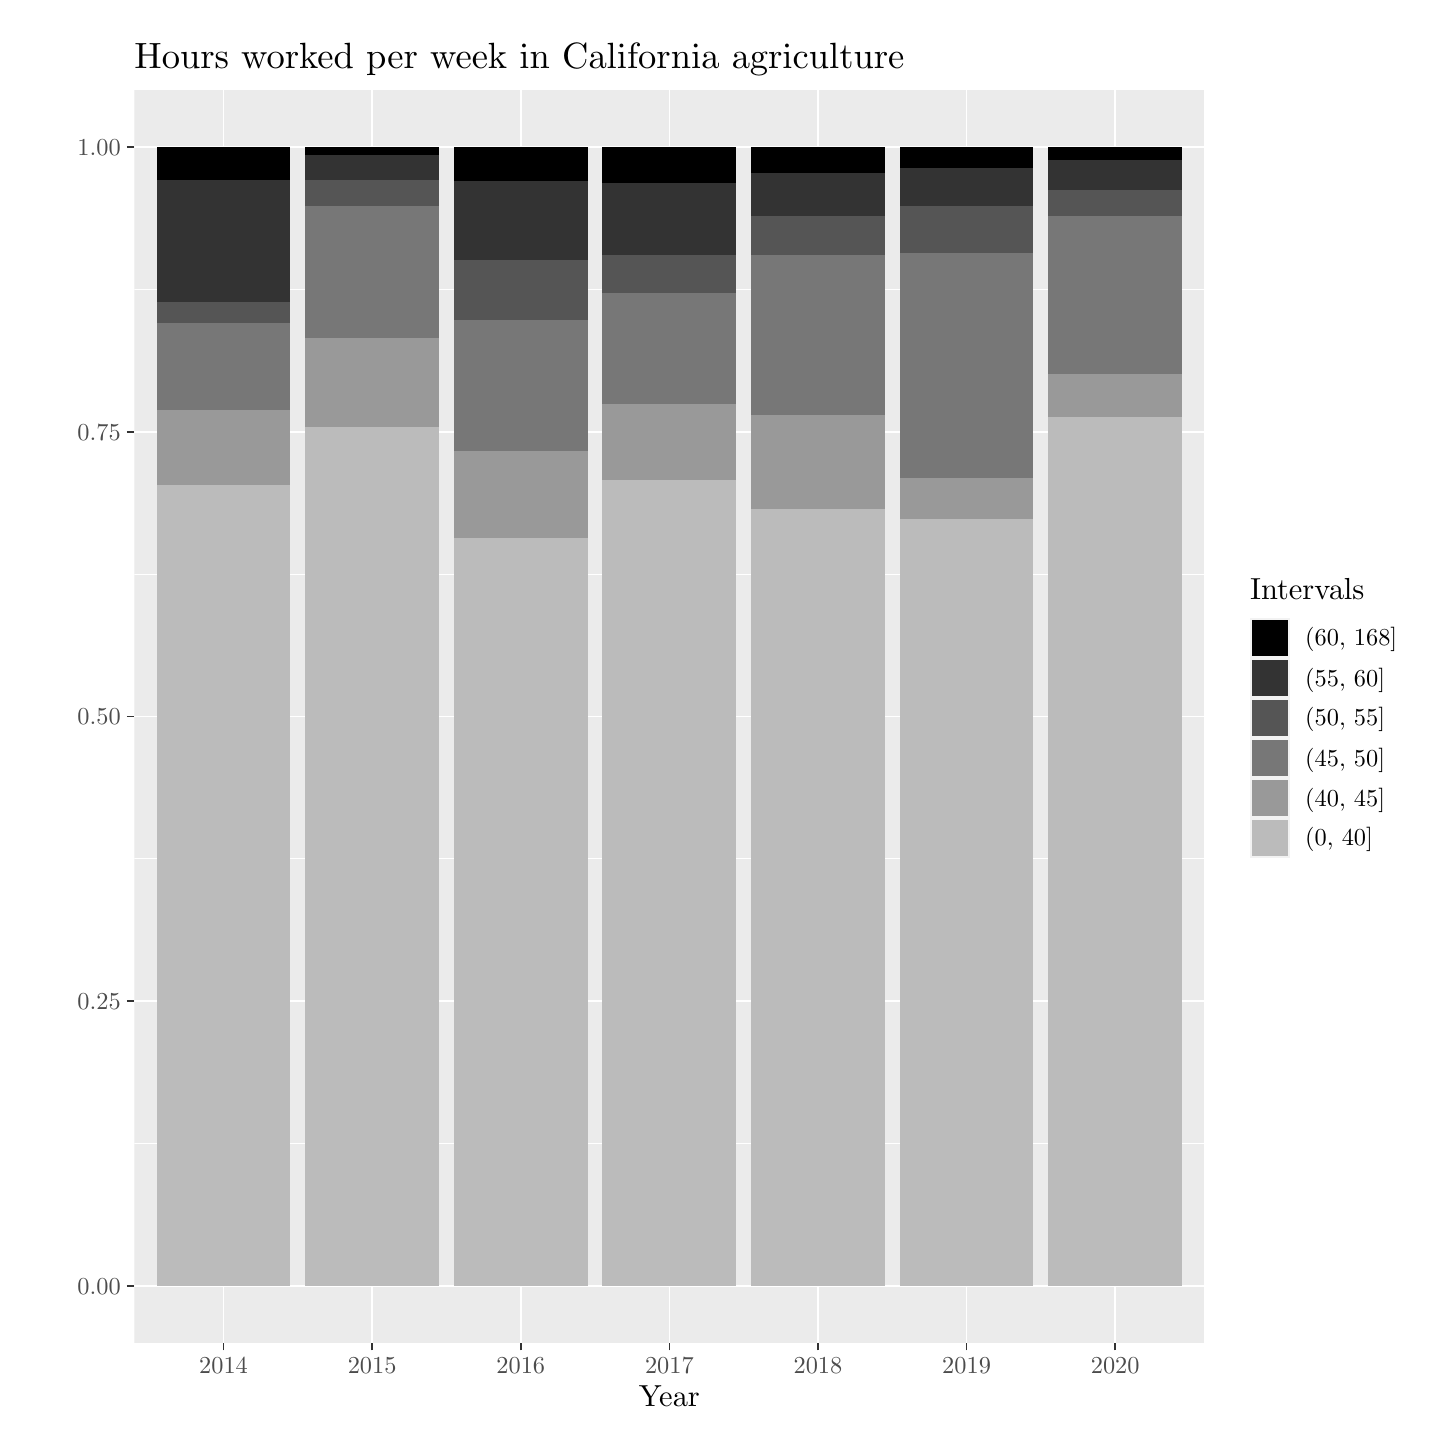
\begin{tikzpicture}[x=1pt,y=1pt]
	\definecolor{fillColor}{RGB}{255,255,255}
	\path[use as bounding box,fill=fillColor,fill opacity=0.00] (0,0) rectangle (505.89,505.89);
	\begin{scope}
		\path[clip] (  0.00,  0.00) rectangle (505.89,505.89);
		\definecolor{drawColor}{RGB}{255,255,255}
		\definecolor{fillColor}{RGB}{255,255,255}

		\path[draw=drawColor,line width= 0.6pt,line join=round,line cap=round,fill=fillColor] (  0.00,  0.00) rectangle (505.89,505.89);
	\end{scope}
	\begin{scope}
		\path[clip] ( 38.56, 30.69) rectangle (425.20,483.23);
		\definecolor{fillColor}{gray}{0.92}

		\path[fill=fillColor] ( 38.56, 30.69) rectangle (425.20,483.23);
		\definecolor{drawColor}{RGB}{255,255,255}

		\path[draw=drawColor,line width= 0.3pt,line join=round] ( 38.56,102.68) --
		(425.20,102.68);

		\path[draw=drawColor,line width= 0.3pt,line join=round] ( 38.56,205.53) --
		(425.20,205.53);

		\path[draw=drawColor,line width= 0.3pt,line join=round] ( 38.56,308.39) --
		(425.20,308.39);

		\path[draw=drawColor,line width= 0.3pt,line join=round] ( 38.56,411.24) --
		(425.20,411.24);

		\path[draw=drawColor,line width= 0.6pt,line join=round] ( 38.56, 51.26) --
		(425.20, 51.26);

		\path[draw=drawColor,line width= 0.6pt,line join=round] ( 38.56,154.11) --
		(425.20,154.11);

		\path[draw=drawColor,line width= 0.6pt,line join=round] ( 38.56,256.96) --
		(425.20,256.96);

		\path[draw=drawColor,line width= 0.6pt,line join=round] ( 38.56,359.81) --
		(425.20,359.81);

		\path[draw=drawColor,line width= 0.6pt,line join=round] ( 38.56,462.66) --
		(425.20,462.66);

		\path[draw=drawColor,line width= 0.6pt,line join=round] ( 70.78, 30.69) --
		( 70.78,483.23);

		\path[draw=drawColor,line width= 0.6pt,line join=round] (124.48, 30.69) --
		(124.48,483.23);

		\path[draw=drawColor,line width= 0.6pt,line join=round] (178.18, 30.69) --
		(178.18,483.23);

		\path[draw=drawColor,line width= 0.6pt,line join=round] (231.88, 30.69) --
		(231.88,483.23);

		\path[draw=drawColor,line width= 0.6pt,line join=round] (285.58, 30.69) --
		(285.58,483.23);

		\path[draw=drawColor,line width= 0.6pt,line join=round] (339.28, 30.69) --
		(339.28,483.23);

		\path[draw=drawColor,line width= 0.6pt,line join=round] (392.98, 30.69) --
		(392.98,483.23);
		\definecolor{fillColor}{RGB}{0,0,0}

		\path[fill=fillColor] ( 46.61,450.95) rectangle ( 94.94,462.66);
		\definecolor{fillColor}{gray}{0.20}

		\path[fill=fillColor] ( 46.61,406.84) rectangle ( 94.94,450.95);
		\definecolor{fillColor}{RGB}{85,85,85}

		\path[fill=fillColor] ( 46.61,399.26) rectangle ( 94.94,406.84);
		\definecolor{fillColor}{RGB}{119,119,119}

		\path[fill=fillColor] ( 46.61,367.56) rectangle ( 94.94,399.26);
		\definecolor{fillColor}{gray}{0.60}

		\path[fill=fillColor] ( 46.61,340.69) rectangle ( 94.94,367.56);
		\definecolor{fillColor}{RGB}{187,187,187}

		\path[fill=fillColor] ( 46.61, 51.26) rectangle ( 94.94,340.69);
		\definecolor{fillColor}{RGB}{0,0,0}

		\path[fill=fillColor] (100.31,459.73) rectangle (148.64,462.66);
		\definecolor{fillColor}{gray}{0.20}

		\path[fill=fillColor] (100.31,450.95) rectangle (148.64,459.73);
		\definecolor{fillColor}{RGB}{85,85,85}

		\path[fill=fillColor] (100.31,441.43) rectangle (148.64,450.95);
		\definecolor{fillColor}{RGB}{119,119,119}

		\path[fill=fillColor] (100.31,393.85) rectangle (148.64,441.43);
		\definecolor{fillColor}{gray}{0.60}

		\path[fill=fillColor] (100.31,361.64) rectangle (148.64,393.85);
		\definecolor{fillColor}{RGB}{187,187,187}

		\path[fill=fillColor] (100.31, 51.26) rectangle (148.64,361.64);
		\definecolor{fillColor}{RGB}{0,0,0}

		\path[fill=fillColor] (154.01,450.33) rectangle (202.34,462.66);
		\definecolor{fillColor}{gray}{0.20}

		\path[fill=fillColor] (154.01,421.95) rectangle (202.34,450.33);
		\definecolor{fillColor}{RGB}{85,85,85}

		\path[fill=fillColor] (154.01,400.37) rectangle (202.34,421.95);
		\definecolor{fillColor}{RGB}{119,119,119}

		\path[fill=fillColor] (154.01,352.87) rectangle (202.34,400.37);
		\definecolor{fillColor}{gray}{0.60}

		\path[fill=fillColor] (154.01,321.42) rectangle (202.34,352.87);
		\definecolor{fillColor}{RGB}{187,187,187}

		\path[fill=fillColor] (154.01, 51.26) rectangle (202.34,321.42);
		\definecolor{fillColor}{RGB}{0,0,0}

		\path[fill=fillColor] (207.71,449.66) rectangle (256.04,462.66);
		\definecolor{fillColor}{gray}{0.20}

		\path[fill=fillColor] (207.71,423.67) rectangle (256.04,449.66);
		\definecolor{fillColor}{RGB}{85,85,85}

		\path[fill=fillColor] (207.71,410.02) rectangle (256.04,423.67);
		\definecolor{fillColor}{RGB}{119,119,119}

		\path[fill=fillColor] (207.71,369.72) rectangle (256.04,410.02);
		\definecolor{fillColor}{gray}{0.60}

		\path[fill=fillColor] (207.71,342.43) rectangle (256.04,369.72);
		\definecolor{fillColor}{RGB}{187,187,187}

		\path[fill=fillColor] (207.71, 51.26) rectangle (256.04,342.43);
		\definecolor{fillColor}{RGB}{0,0,0}

		\path[fill=fillColor] (261.41,453.37) rectangle (309.74,462.66);
		\definecolor{fillColor}{gray}{0.20}

		\path[fill=fillColor] (261.41,437.88) rectangle (309.74,453.37);
		\definecolor{fillColor}{RGB}{85,85,85}

		\path[fill=fillColor] (261.41,423.63) rectangle (309.74,437.88);
		\definecolor{fillColor}{RGB}{119,119,119}

		\path[fill=fillColor] (261.41,366.01) rectangle (309.74,423.63);
		\definecolor{fillColor}{gray}{0.60}

		\path[fill=fillColor] (261.41,331.93) rectangle (309.74,366.01);
		\definecolor{fillColor}{RGB}{187,187,187}

		\path[fill=fillColor] (261.41, 51.26) rectangle (309.74,331.93);
		\definecolor{fillColor}{RGB}{0,0,0}

		\path[fill=fillColor] (315.11,455.13) rectangle (363.44,462.66);
		\definecolor{fillColor}{gray}{0.20}

		\path[fill=fillColor] (315.11,441.31) rectangle (363.44,455.13);
		\definecolor{fillColor}{RGB}{85,85,85}

		\path[fill=fillColor] (315.11,424.35) rectangle (363.44,441.31);
		\definecolor{fillColor}{RGB}{119,119,119}

		\path[fill=fillColor] (315.11,343.32) rectangle (363.44,424.35);
		\definecolor{fillColor}{gray}{0.60}

		\path[fill=fillColor] (315.11,328.25) rectangle (363.44,343.32);
		\definecolor{fillColor}{RGB}{187,187,187}

		\path[fill=fillColor] (315.11, 51.26) rectangle (363.44,328.25);
		\definecolor{fillColor}{RGB}{0,0,0}

		\path[fill=fillColor] (368.81,457.89) rectangle (417.14,462.66);
		\definecolor{fillColor}{gray}{0.20}

		\path[fill=fillColor] (368.81,447.39) rectangle (417.14,457.89);
		\definecolor{fillColor}{RGB}{85,85,85}

		\path[fill=fillColor] (368.81,437.84) rectangle (417.14,447.39);
		\definecolor{fillColor}{RGB}{119,119,119}

		\path[fill=fillColor] (368.81,380.57) rectangle (417.14,437.84);
		\definecolor{fillColor}{gray}{0.60}

		\path[fill=fillColor] (368.81,365.30) rectangle (417.14,380.57);
		\definecolor{fillColor}{RGB}{187,187,187}

		\path[fill=fillColor] (368.81, 51.26) rectangle (417.14,365.30);
	\end{scope}
	\begin{scope}
		\path[clip] (  0.00,  0.00) rectangle (505.89,505.89);
		\definecolor{drawColor}{gray}{0.30}

		\node[text=drawColor,anchor=base east,inner sep=0pt, outer sep=0pt, scale=  0.88] at ( 33.61, 48.23) {0.00};

		\node[text=drawColor,anchor=base east,inner sep=0pt, outer sep=0pt, scale=  0.88] at ( 33.61,151.08) {0.25};

		\node[text=drawColor,anchor=base east,inner sep=0pt, outer sep=0pt, scale=  0.88] at ( 33.61,253.93) {0.50};

		\node[text=drawColor,anchor=base east,inner sep=0pt, outer sep=0pt, scale=  0.88] at ( 33.61,356.78) {0.75};

		\node[text=drawColor,anchor=base east,inner sep=0pt, outer sep=0pt, scale=  0.88] at ( 33.61,459.63) {1.00};
	\end{scope}
	\begin{scope}
		\path[clip] (  0.00,  0.00) rectangle (505.89,505.89);
		\definecolor{drawColor}{gray}{0.20}

		\path[draw=drawColor,line width= 0.6pt,line join=round] ( 35.81, 51.26) --
		( 38.56, 51.26);

		\path[draw=drawColor,line width= 0.6pt,line join=round] ( 35.81,154.11) --
		( 38.56,154.11);

		\path[draw=drawColor,line width= 0.6pt,line join=round] ( 35.81,256.96) --
		( 38.56,256.96);

		\path[draw=drawColor,line width= 0.6pt,line join=round] ( 35.81,359.81) --
		( 38.56,359.81);

		\path[draw=drawColor,line width= 0.6pt,line join=round] ( 35.81,462.66) --
		( 38.56,462.66);
	\end{scope}
	\begin{scope}
		\path[clip] (  0.00,  0.00) rectangle (505.89,505.89);
		\definecolor{drawColor}{gray}{0.20}

		\path[draw=drawColor,line width= 0.6pt,line join=round] ( 70.78, 27.94) --
		( 70.78, 30.69);

		\path[draw=drawColor,line width= 0.6pt,line join=round] (124.48, 27.94) --
		(124.48, 30.69);

		\path[draw=drawColor,line width= 0.6pt,line join=round] (178.18, 27.94) --
		(178.18, 30.69);

		\path[draw=drawColor,line width= 0.6pt,line join=round] (231.88, 27.94) --
		(231.88, 30.69);

		\path[draw=drawColor,line width= 0.6pt,line join=round] (285.58, 27.94) --
		(285.58, 30.69);

		\path[draw=drawColor,line width= 0.6pt,line join=round] (339.28, 27.94) --
		(339.28, 30.69);

		\path[draw=drawColor,line width= 0.6pt,line join=round] (392.98, 27.94) --
		(392.98, 30.69);
	\end{scope}
	\begin{scope}
		\path[clip] (  0.00,  0.00) rectangle (505.89,505.89);
		\definecolor{drawColor}{gray}{0.30}

		\node[text=drawColor,anchor=base,inner sep=0pt, outer sep=0pt, scale=  0.88] at ( 70.78, 19.68) {2014};

		\node[text=drawColor,anchor=base,inner sep=0pt, outer sep=0pt, scale=  0.88] at (124.48, 19.68) {2015};

		\node[text=drawColor,anchor=base,inner sep=0pt, outer sep=0pt, scale=  0.88] at (178.18, 19.68) {2016};

		\node[text=drawColor,anchor=base,inner sep=0pt, outer sep=0pt, scale=  0.88] at (231.88, 19.68) {2017};

		\node[text=drawColor,anchor=base,inner sep=0pt, outer sep=0pt, scale=  0.88] at (285.58, 19.68) {2018};

		\node[text=drawColor,anchor=base,inner sep=0pt, outer sep=0pt, scale=  0.88] at (339.28, 19.68) {2019};

		\node[text=drawColor,anchor=base,inner sep=0pt, outer sep=0pt, scale=  0.88] at (392.98, 19.68) {2020};
	\end{scope}
	\begin{scope}
		\path[clip] (  0.00,  0.00) rectangle (505.89,505.89);
		\definecolor{drawColor}{RGB}{0,0,0}

		\node[text=drawColor,anchor=base,inner sep=0pt, outer sep=0pt, scale=  1.10] at (231.88,  7.64) {Year};
	\end{scope}
	\begin{scope}
		\path[clip] (  0.00,  0.00) rectangle (505.89,505.89);
		\definecolor{fillColor}{RGB}{255,255,255}

		\path[fill=fillColor] (436.20,200.49) rectangle (500.39,313.43);
	\end{scope}
	\begin{scope}
		\path[clip] (  0.00,  0.00) rectangle (505.89,505.89);
		\definecolor{drawColor}{RGB}{0,0,0}

		\node[text=drawColor,anchor=base west,inner sep=0pt, outer sep=0pt, scale=  1.10] at (441.70,299.28) {Intervals};
	\end{scope}
	\begin{scope}
		\path[clip] (  0.00,  0.00) rectangle (505.89,505.89);
		\definecolor{fillColor}{gray}{0.95}

		\path[fill=fillColor] (441.70,278.26) rectangle (456.15,292.71);
	\end{scope}
	\begin{scope}
		\path[clip] (  0.00,  0.00) rectangle (505.89,505.89);
		\definecolor{fillColor}{RGB}{0,0,0}

		\path[fill=fillColor] (442.41,278.97) rectangle (455.44,292.00);
	\end{scope}
	\begin{scope}
		\path[clip] (  0.00,  0.00) rectangle (505.89,505.89);
		\definecolor{fillColor}{gray}{0.95}

		\path[fill=fillColor] (441.70,263.81) rectangle (456.15,278.26);
	\end{scope}
	\begin{scope}
		\path[clip] (  0.00,  0.00) rectangle (505.89,505.89);
		\definecolor{fillColor}{gray}{0.20}

		\path[fill=fillColor] (442.41,264.52) rectangle (455.44,277.55);
	\end{scope}
	\begin{scope}
		\path[clip] (  0.00,  0.00) rectangle (505.89,505.89);
		\definecolor{fillColor}{gray}{0.95}

		\path[fill=fillColor] (441.70,249.35) rectangle (456.15,263.81);
	\end{scope}
	\begin{scope}
		\path[clip] (  0.00,  0.00) rectangle (505.89,505.89);
		\definecolor{fillColor}{RGB}{85,85,85}

		\path[fill=fillColor] (442.41,250.06) rectangle (455.44,263.09);
	\end{scope}
	\begin{scope}
		\path[clip] (  0.00,  0.00) rectangle (505.89,505.89);
		\definecolor{fillColor}{gray}{0.95}

		\path[fill=fillColor] (441.70,234.90) rectangle (456.15,249.35);
	\end{scope}
	\begin{scope}
		\path[clip] (  0.00,  0.00) rectangle (505.89,505.89);
		\definecolor{fillColor}{RGB}{119,119,119}

		\path[fill=fillColor] (442.41,235.61) rectangle (455.44,248.64);
	\end{scope}
	\begin{scope}
		\path[clip] (  0.00,  0.00) rectangle (505.89,505.89);
		\definecolor{fillColor}{gray}{0.95}

		\path[fill=fillColor] (441.70,220.44) rectangle (456.15,234.90);
	\end{scope}
	\begin{scope}
		\path[clip] (  0.00,  0.00) rectangle (505.89,505.89);
		\definecolor{fillColor}{gray}{0.60}

		\path[fill=fillColor] (442.41,221.16) rectangle (455.44,234.19);
	\end{scope}
	\begin{scope}
		\path[clip] (  0.00,  0.00) rectangle (505.89,505.89);
		\definecolor{fillColor}{gray}{0.95}

		\path[fill=fillColor] (441.70,205.99) rectangle (456.15,220.44);
	\end{scope}
	\begin{scope}
		\path[clip] (  0.00,  0.00) rectangle (505.89,505.89);
		\definecolor{fillColor}{RGB}{187,187,187}

		\path[fill=fillColor] (442.41,206.70) rectangle (455.44,219.73);
	\end{scope}
	\begin{scope}
		\path[clip] (  0.00,  0.00) rectangle (505.89,505.89);
		\definecolor{drawColor}{RGB}{0,0,0}

		\node[text=drawColor,anchor=base west,inner sep=0pt, outer sep=0pt, scale=  0.88] at (461.65,282.46) {(60, 168]};
	\end{scope}
	\begin{scope}
		\path[clip] (  0.00,  0.00) rectangle (505.89,505.89);
		\definecolor{drawColor}{RGB}{0,0,0}

		\node[text=drawColor,anchor=base west,inner sep=0pt, outer sep=0pt, scale=  0.88] at (461.65,268.00) {(55, 60]};
	\end{scope}
	\begin{scope}
		\path[clip] (  0.00,  0.00) rectangle (505.89,505.89);
		\definecolor{drawColor}{RGB}{0,0,0}

		\node[text=drawColor,anchor=base west,inner sep=0pt, outer sep=0pt, scale=  0.88] at (461.65,253.55) {(50, 55]};
	\end{scope}
	\begin{scope}
		\path[clip] (  0.00,  0.00) rectangle (505.89,505.89);
		\definecolor{drawColor}{RGB}{0,0,0}

		\node[text=drawColor,anchor=base west,inner sep=0pt, outer sep=0pt, scale=  0.88] at (461.65,239.09) {(45, 50]};
	\end{scope}
	\begin{scope}
		\path[clip] (  0.00,  0.00) rectangle (505.89,505.89);
		\definecolor{drawColor}{RGB}{0,0,0}

		\node[text=drawColor,anchor=base west,inner sep=0pt, outer sep=0pt, scale=  0.88] at (461.65,224.64) {(40, 45]};
	\end{scope}
	\begin{scope}
		\path[clip] (  0.00,  0.00) rectangle (505.89,505.89);
		\definecolor{drawColor}{RGB}{0,0,0}

		\node[text=drawColor,anchor=base west,inner sep=0pt, outer sep=0pt, scale=  0.88] at (461.65,210.19) {(0, 40]};
	\end{scope}
	\begin{scope}
		\path[clip] (  0.00,  0.00) rectangle (505.89,505.89);
		\definecolor{drawColor}{RGB}{0,0,0}

		\node[text=drawColor,anchor=base west,inner sep=0pt, outer sep=0pt, scale=  1.32] at ( 38.56,491.30) {Hours worked per week in California agriculture};
	\end{scope}
\end{tikzpicture}

    }
    \begin{table}[!h]

    \caption{Summary Statistics by industry for CA 2018-2019}
    \centering
    \begin{tabular}[t]{|l|>{\centering\arraybackslash}b{2.5cm}|>{\centering\arraybackslash}b{2.5cm}|}
        \hline
                             & Agriculture & Food services and drinking places \\
        \hline
        Hours                & 41.4        & 32.4                              \\
        \hline
        Age                  & 45.2        & 33.9                              \\
        \hline
        High school graduate & 0.521       & 0.787                             \\
        \hline
        Percentage male      & 0.714       & 0.491                             \\
        \hline
        Percentage white     & 0.911       & 0.747                             \\
        \hline
        Married              & 0.589       & 0.301                             \\
        \hline
        Citizenship          & 0.530       & 0.757                             \\
        \hline
        Union membership     & 0.913       & 0.968                             \\
        \hline
        Hourly wage          & 13.40       & 13.50                             \\
        \hline
        Weekly earnings      & 681         & 562                               \\
        \hline
        Sample size          & 2202        & 7333                              \\
        \hline
    \end{tabular}
\end{table}
\end{center}

\section{Empirical Strategy}
\subsection{Difference-in-Differences}
I use difference-in-differences (DiD) to study the impact of overtime legislation on hourly wages, characterized by the following formula:
\[y_{igt} = \alpha_g + \delta_t + X_{igt}\gamma + \beta_1D_{1gt} + \beta_2D_{2gt} + \epsilon_{igt}\]
Here, $\alpha_g$ and $\delta_t$ are group and year fixed effects, while $X_{igt}$ is a vector of demographic characteristics similar to those chosen in Trejo's (1991) overtime study—namely, age, sex, race, location, high school graduation status, and marital status. I run regressions both with and without these characteristics. Finally, $D_{1gt}$ and $D_{2gt}$ are dummies which take on a value of 1 for agricultural workers starting from the first and second year of treatment, respectively. The coefficients on these dummies are the DiD estimates of the 2019 and 2020 reduction in standard hours.\par
Four choices of dependent variable $y_{igt}$ are considered, two of which are the hourly wage and the log-transformed hourly wage. The other two dependent variables exploit the different schedules of overtime and minimum wage requirements for businesses with 25 or fewer employees (U25) and businesses with greater than 25 employees (O25). By tracking the proportion of workers working at the U25 and O25 minimum wage between the treated and control groups, we should expect to see similar trends prior to the overtime policy. In 2019 and 2020, there should be a divergence present in the O25 proportion and not the U25 proportion, representing a reduction in wages due to the overtime policy. \par

\bgroup
\def\arraystretch{1.25}
\begin{table}
    \centering
    \caption{CA Minimum Wage and Agricultural Overtime Changes}
    \label{}
    \begin{tabular}{||c| c c | c c||}
        \hline
        Year & \multicolumn{2}{c|}{Minimum Wage (hour)} & \multicolumn{2}{c||}{Overtime (day/week)}                                \\
             & $\leq 25$ emp.                           & $> 25$ emp.                               & $\leq 25$ emp. & $> 25$ emp. \\
        \hline
        \hline
        2016 & \$10.00                                  & \$10.00                                   & 10/60          & 10/60       \\
        \hline
        2017 & \$10.00                                  & \$10.50                                   & 10/60          & 10/60       \\
        \hline
        2018 & \$10.50                                  & \$11.00                                   & 10/60          & 10/60       \\
        \hline
        2019 & \$11.00                                  & \$12.00                                   & 10/60          & 9.5/55      \\
        \hline
        2020 & \$12.00                                  & \$13.00                                   & 10/60          & 9/50        \\
        \hline
    \end{tabular}
\end{table}
\egroup

For all of the DiD regressions, I choose control groups based on similarity of pre-treatment trends in average hourly wages and proportion working at either minimum wage. Because multiple minimum wage increases occurred within the pre-treatment window, this ensures that these changes did not have heterogeneous effects on the treated and control groups in 2019 and 2020, meaning differences are solely due to overtime policy. The chosen control groups were retail and restaurant cashiers, waiters/waitresses, and restaurant food preparation workers. Figure 1 displays the trends in wages and proportions at the O25 and U25 minimum wages, giving a visual verification of the parallel trends assumption.

\begin{landscape}
    \begin{figure}
        \caption{Difference-in-Differences Parallel Trends Plots}
        \label{}
        \vspace*{\fill}
        \centering
        \scalebox{0.5}{
            % Created by tikzDevice version 0.12.3.1 on 2021-12-16 11:00:05
% !TEX encoding = UTF-8 Unicode
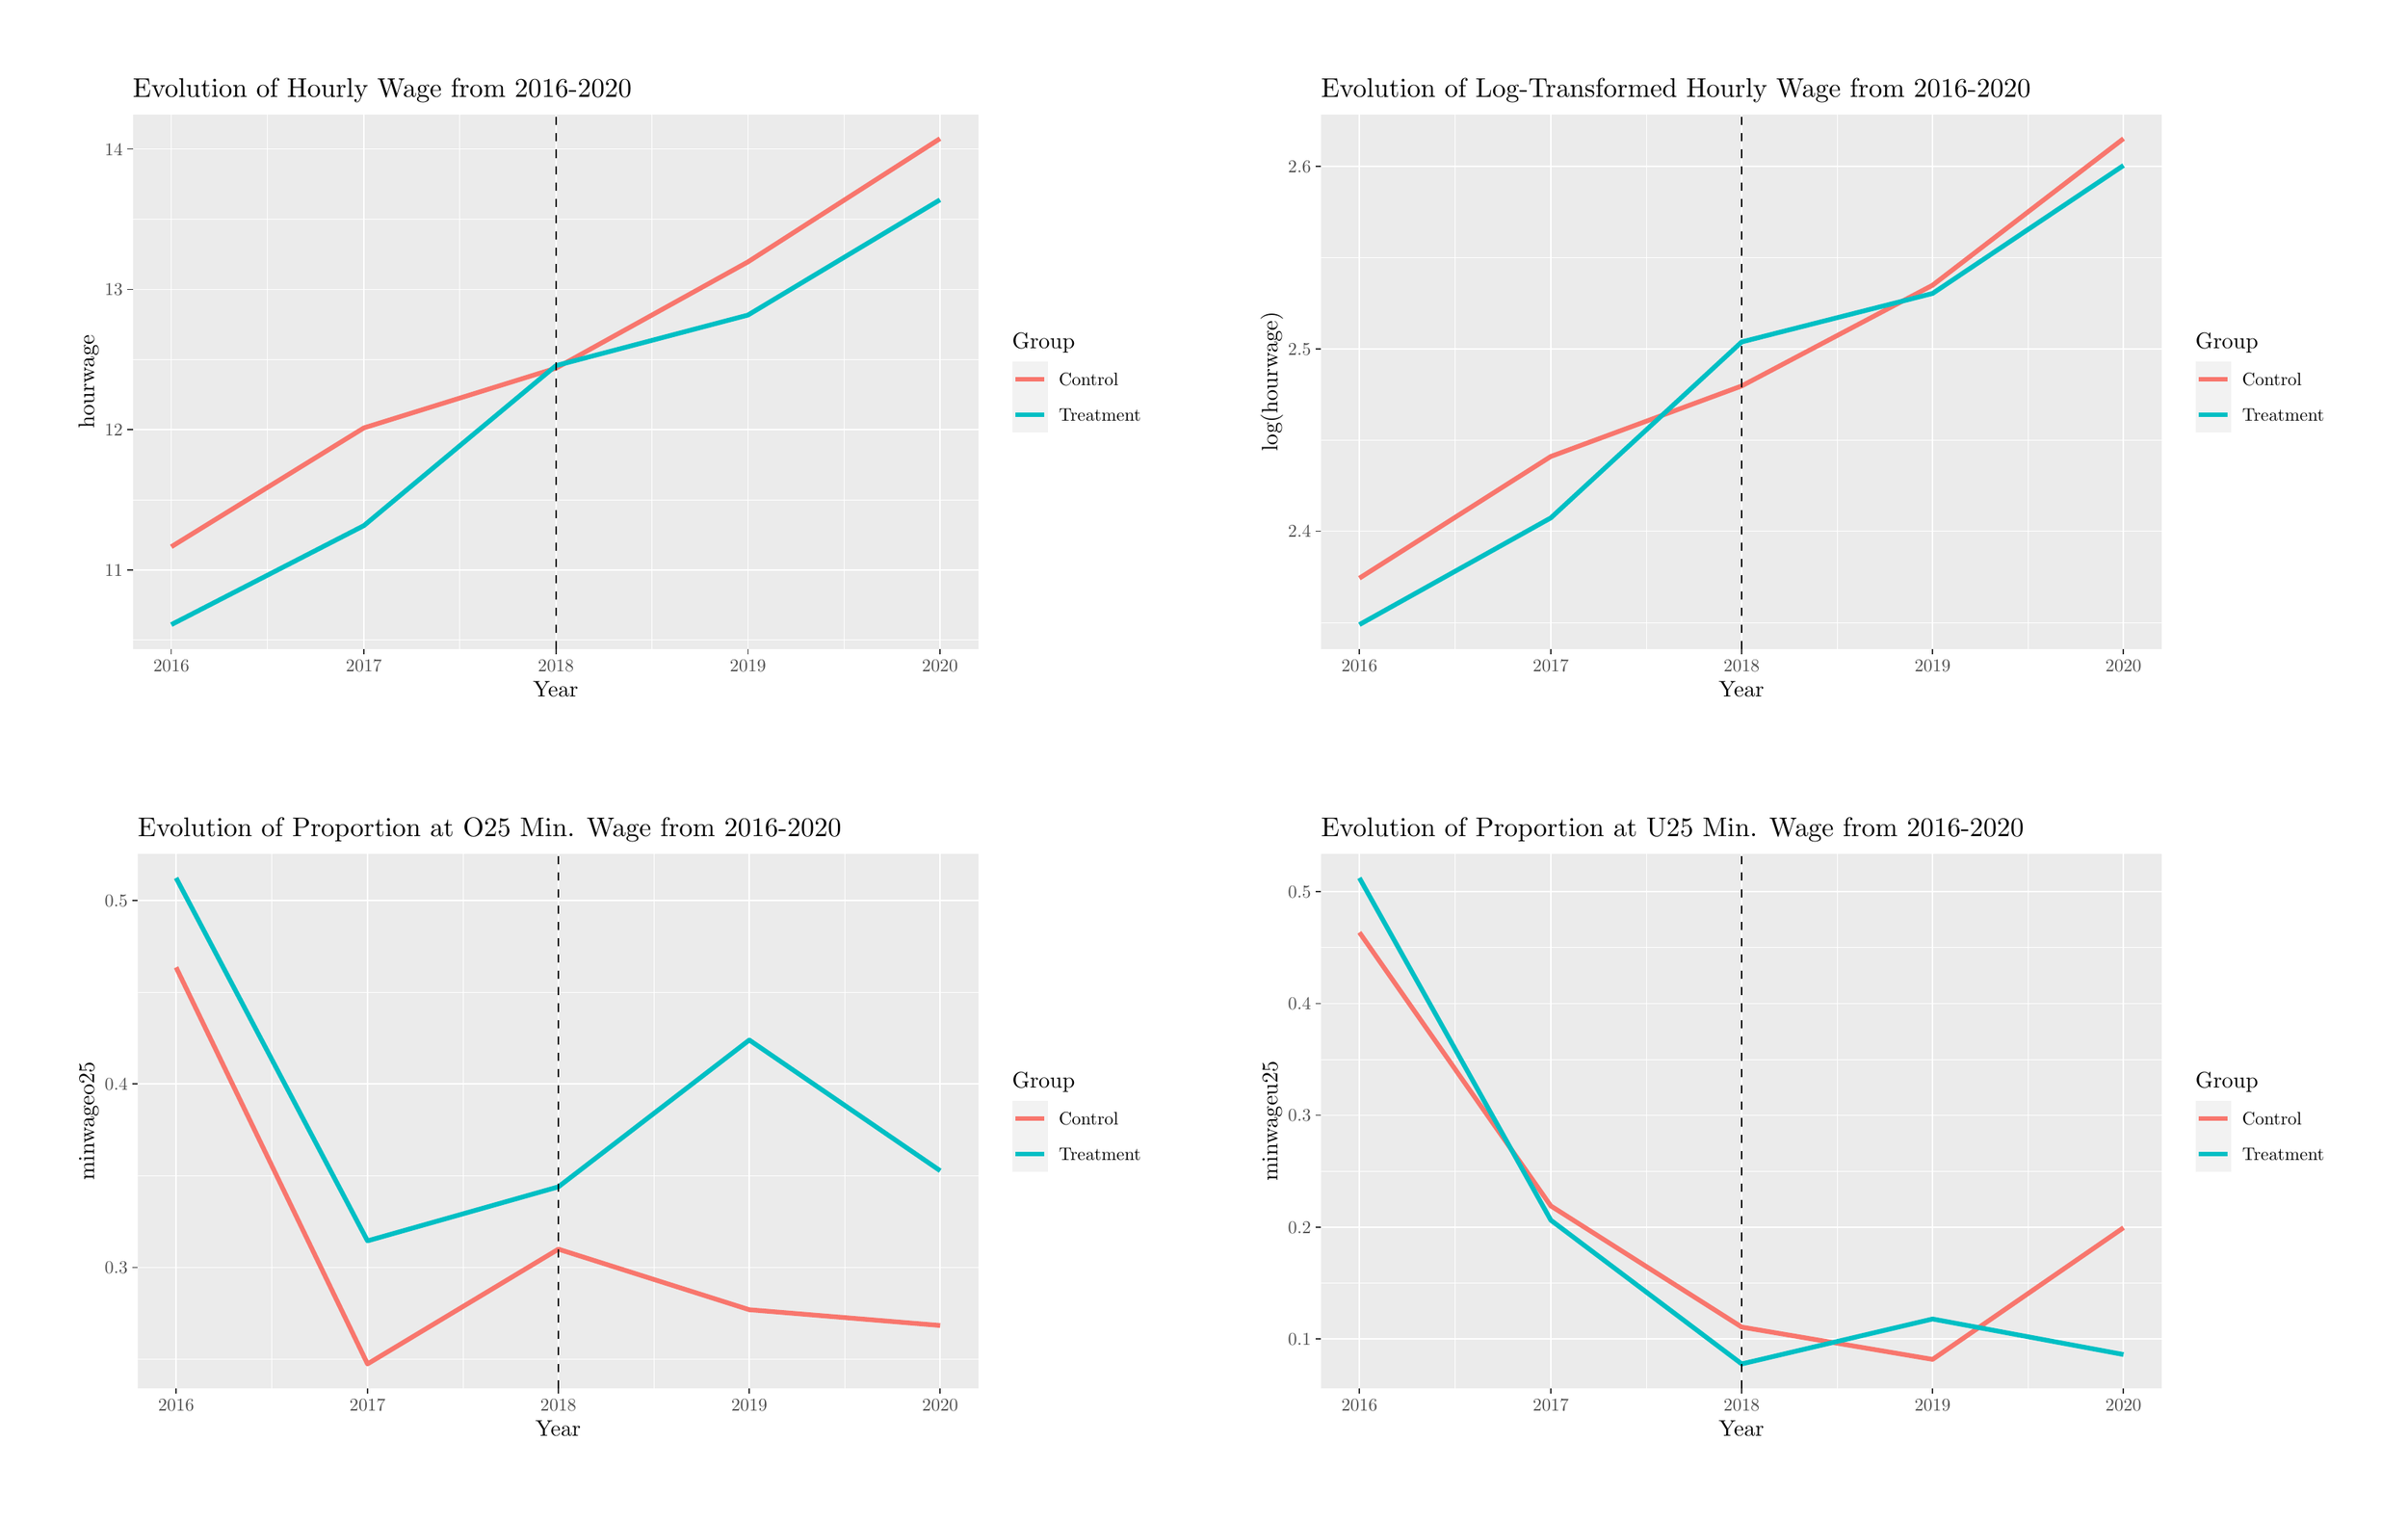
\begin{tikzpicture}[x=1pt,y=1pt]
\definecolor{fillColor}{RGB}{255,255,255}
\path[use as bounding box,fill=fillColor,fill opacity=0.00] (0,0) rectangle (1156.32,722.70);
\begin{scope}
\path[clip] (  0.00,361.35) rectangle (578.16,722.70);
\definecolor{drawColor}{RGB}{255,255,255}
\definecolor{fillColor}{RGB}{255,255,255}

\path[draw=drawColor,line width= 0.6pt,line join=round,line cap=round,fill=fillColor] (  0.00,361.35) rectangle (578.16,722.70);
\end{scope}
\begin{scope}
\path[clip] ( 54.93,415.52) rectangle (468.05,676.81);
\definecolor{fillColor}{gray}{0.92}

\path[fill=fillColor] ( 54.93,415.52) rectangle (468.05,676.81);
\definecolor{drawColor}{RGB}{255,255,255}

\path[draw=drawColor,line width= 0.3pt,line join=round] ( 54.93,419.81) --
	(468.05,419.81);

\path[draw=drawColor,line width= 0.3pt,line join=round] ( 54.93,488.39) --
	(468.05,488.39);

\path[draw=drawColor,line width= 0.3pt,line join=round] ( 54.93,556.97) --
	(468.05,556.97);

\path[draw=drawColor,line width= 0.3pt,line join=round] ( 54.93,625.55) --
	(468.05,625.55);

\path[draw=drawColor,line width= 0.3pt,line join=round] (120.75,415.52) --
	(120.75,676.81);

\path[draw=drawColor,line width= 0.3pt,line join=round] (214.71,415.52) --
	(214.71,676.81);

\path[draw=drawColor,line width= 0.3pt,line join=round] (308.53,415.52) --
	(308.53,676.81);

\path[draw=drawColor,line width= 0.3pt,line join=round] (402.36,415.52) --
	(402.36,676.81);

\path[draw=drawColor,line width= 0.6pt,line join=round] ( 54.93,454.10) --
	(468.05,454.10);

\path[draw=drawColor,line width= 0.6pt,line join=round] ( 54.93,522.68) --
	(468.05,522.68);

\path[draw=drawColor,line width= 0.6pt,line join=round] ( 54.93,591.26) --
	(468.05,591.26);

\path[draw=drawColor,line width= 0.6pt,line join=round] ( 54.93,659.83) --
	(468.05,659.83);

\path[draw=drawColor,line width= 0.6pt,line join=round] ( 73.71,415.52) --
	( 73.71,676.81);

\path[draw=drawColor,line width= 0.6pt,line join=round] (167.79,415.52) --
	(167.79,676.81);

\path[draw=drawColor,line width= 0.6pt,line join=round] (261.62,415.52) --
	(261.62,676.81);

\path[draw=drawColor,line width= 0.6pt,line join=round] (355.45,415.52) --
	(355.45,676.81);

\path[draw=drawColor,line width= 0.6pt,line join=round] (449.27,415.52) --
	(449.27,676.81);
\definecolor{drawColor}{RGB}{248,118,109}

\path[draw=drawColor,line width= 2.3pt,line join=round] ( 73.71,465.46) --
	(167.79,523.54) --
	(261.62,552.72) --
	(355.45,604.68) --
	(449.27,664.93);
\definecolor{drawColor}{RGB}{0,191,196}

\path[draw=drawColor,line width= 2.3pt,line join=round] ( 73.71,427.39) --
	(167.79,475.77) --
	(261.62,553.97) --
	(355.45,578.69) --
	(449.27,635.03);
\definecolor{drawColor}{RGB}{0,0,0}

\path[draw=drawColor,line width= 0.6pt,dash pattern=on 4pt off 4pt ,line join=round] (261.62,415.52) -- (261.62,676.81);
\end{scope}
\begin{scope}
\path[clip] (  0.00,  0.00) rectangle (1156.32,722.70);
\definecolor{drawColor}{gray}{0.30}

\node[text=drawColor,anchor=base east,inner sep=0pt, outer sep=0pt, scale=  0.88] at ( 49.98,451.07) {11};

\node[text=drawColor,anchor=base east,inner sep=0pt, outer sep=0pt, scale=  0.88] at ( 49.98,519.65) {12};

\node[text=drawColor,anchor=base east,inner sep=0pt, outer sep=0pt, scale=  0.88] at ( 49.98,588.23) {13};

\node[text=drawColor,anchor=base east,inner sep=0pt, outer sep=0pt, scale=  0.88] at ( 49.98,656.80) {14};
\end{scope}
\begin{scope}
\path[clip] (  0.00,  0.00) rectangle (1156.32,722.70);
\definecolor{drawColor}{gray}{0.20}

\path[draw=drawColor,line width= 0.6pt,line join=round] ( 52.18,454.10) --
	( 54.93,454.10);

\path[draw=drawColor,line width= 0.6pt,line join=round] ( 52.18,522.68) --
	( 54.93,522.68);

\path[draw=drawColor,line width= 0.6pt,line join=round] ( 52.18,591.26) --
	( 54.93,591.26);

\path[draw=drawColor,line width= 0.6pt,line join=round] ( 52.18,659.83) --
	( 54.93,659.83);
\end{scope}
\begin{scope}
\path[clip] (  0.00,  0.00) rectangle (1156.32,722.70);
\definecolor{drawColor}{gray}{0.20}

\path[draw=drawColor,line width= 0.6pt,line join=round] ( 73.71,412.77) --
	( 73.71,415.52);

\path[draw=drawColor,line width= 0.6pt,line join=round] (167.79,412.77) --
	(167.79,415.52);

\path[draw=drawColor,line width= 0.6pt,line join=round] (261.62,412.77) --
	(261.62,415.52);

\path[draw=drawColor,line width= 0.6pt,line join=round] (355.45,412.77) --
	(355.45,415.52);

\path[draw=drawColor,line width= 0.6pt,line join=round] (449.27,412.77) --
	(449.27,415.52);
\end{scope}
\begin{scope}
\path[clip] (  0.00,  0.00) rectangle (1156.32,722.70);
\definecolor{drawColor}{gray}{0.30}

\node[text=drawColor,anchor=base,inner sep=0pt, outer sep=0pt, scale=  0.88] at ( 73.71,404.51) {2016};

\node[text=drawColor,anchor=base,inner sep=0pt, outer sep=0pt, scale=  0.88] at (167.79,404.51) {2017};

\node[text=drawColor,anchor=base,inner sep=0pt, outer sep=0pt, scale=  0.88] at (261.62,404.51) {2018};

\node[text=drawColor,anchor=base,inner sep=0pt, outer sep=0pt, scale=  0.88] at (355.45,404.51) {2019};

\node[text=drawColor,anchor=base,inner sep=0pt, outer sep=0pt, scale=  0.88] at (449.27,404.51) {2020};
\end{scope}
\begin{scope}
\path[clip] (  0.00,  0.00) rectangle (1156.32,722.70);
\definecolor{drawColor}{RGB}{0,0,0}

\node[text=drawColor,anchor=base,inner sep=0pt, outer sep=0pt, scale=  1.10] at (261.49,392.21) {Year};
\end{scope}
\begin{scope}
\path[clip] (  0.00,  0.00) rectangle (1156.32,722.70);
\definecolor{drawColor}{RGB}{0,0,0}

\node[text=drawColor,rotate= 90.00,anchor=base,inner sep=0pt, outer sep=0pt, scale=  1.10] at ( 36.03,546.16) {hourwage};
\end{scope}
\begin{scope}
\path[clip] (  0.00,  0.00) rectangle (1156.32,722.70);
\definecolor{fillColor}{RGB}{255,255,255}

\path[fill=fillColor] (479.05,515.71) rectangle (549.71,576.62);
\end{scope}
\begin{scope}
\path[clip] (  0.00,  0.00) rectangle (1156.32,722.70);
\definecolor{drawColor}{RGB}{0,0,0}

\node[text=drawColor,anchor=base west,inner sep=0pt, outer sep=0pt, scale=  1.10] at (484.55,562.47) {Group};
\end{scope}
\begin{scope}
\path[clip] (  0.00,  0.00) rectangle (1156.32,722.70);
\definecolor{fillColor}{gray}{0.95}

\path[fill=fillColor] (484.55,538.56) rectangle (501.89,555.90);
\end{scope}
\begin{scope}
\path[clip] (  0.00,  0.00) rectangle (1156.32,722.70);
\definecolor{drawColor}{RGB}{248,118,109}

\path[draw=drawColor,line width= 2.3pt,line join=round] (486.28,547.23) -- (500.16,547.23);
\end{scope}
\begin{scope}
\path[clip] (  0.00,  0.00) rectangle (1156.32,722.70);
\definecolor{fillColor}{gray}{0.95}

\path[fill=fillColor] (484.55,521.21) rectangle (501.89,538.56);
\end{scope}
\begin{scope}
\path[clip] (  0.00,  0.00) rectangle (1156.32,722.70);
\definecolor{drawColor}{RGB}{0,191,196}

\path[draw=drawColor,line width= 2.3pt,line join=round] (486.28,529.88) -- (500.16,529.88);
\end{scope}
\begin{scope}
\path[clip] (  0.00,  0.00) rectangle (1156.32,722.70);
\definecolor{drawColor}{RGB}{0,0,0}

\node[text=drawColor,anchor=base west,inner sep=0pt, outer sep=0pt, scale=  0.88] at (507.39,544.20) {Control};
\end{scope}
\begin{scope}
\path[clip] (  0.00,  0.00) rectangle (1156.32,722.70);
\definecolor{drawColor}{RGB}{0,0,0}

\node[text=drawColor,anchor=base west,inner sep=0pt, outer sep=0pt, scale=  0.88] at (507.39,526.85) {Treatment};
\end{scope}
\begin{scope}
\path[clip] (  0.00,  0.00) rectangle (1156.32,722.70);
\definecolor{drawColor}{RGB}{0,0,0}

\node[text=drawColor,anchor=base west,inner sep=0pt, outer sep=0pt, scale=  1.32] at ( 54.93,685.16) {Evolution of Hourly Wage from 2016-2020};
\end{scope}
\begin{scope}
\path[clip] (578.16,361.35) rectangle (1156.32,722.70);
\definecolor{drawColor}{RGB}{255,255,255}
\definecolor{fillColor}{RGB}{255,255,255}

\path[draw=drawColor,line width= 0.6pt,line join=round,line cap=round,fill=fillColor] (578.16,361.35) rectangle (1156.32,722.70);
\end{scope}
\begin{scope}
\path[clip] (635.54,415.52) rectangle (1046.21,676.81);
\definecolor{fillColor}{gray}{0.92}

\path[fill=fillColor] (635.54,415.52) rectangle (1046.21,676.81);
\definecolor{drawColor}{RGB}{255,255,255}

\path[draw=drawColor,line width= 0.3pt,line join=round] (635.54,428.43) --
	(1046.21,428.43);

\path[draw=drawColor,line width= 0.3pt,line join=round] (635.54,517.63) --
	(1046.21,517.63);

\path[draw=drawColor,line width= 0.3pt,line join=round] (635.54,606.83) --
	(1046.21,606.83);

\path[draw=drawColor,line width= 0.3pt,line join=round] (700.97,415.52) --
	(700.97,676.81);

\path[draw=drawColor,line width= 0.3pt,line join=round] (794.37,415.52) --
	(794.37,676.81);

\path[draw=drawColor,line width= 0.3pt,line join=round] (887.64,415.52) --
	(887.64,676.81);

\path[draw=drawColor,line width= 0.3pt,line join=round] (980.91,415.52) --
	(980.91,676.81);

\path[draw=drawColor,line width= 0.6pt,line join=round] (635.54,473.03) --
	(1046.21,473.03);

\path[draw=drawColor,line width= 0.6pt,line join=round] (635.54,562.23) --
	(1046.21,562.23);

\path[draw=drawColor,line width= 0.6pt,line join=round] (635.54,651.43) --
	(1046.21,651.43);

\path[draw=drawColor,line width= 0.6pt,line join=round] (654.20,415.52) --
	(654.20,676.81);

\path[draw=drawColor,line width= 0.6pt,line join=round] (747.73,415.52) --
	(747.73,676.81);

\path[draw=drawColor,line width= 0.6pt,line join=round] (841.00,415.52) --
	(841.00,676.81);

\path[draw=drawColor,line width= 0.6pt,line join=round] (934.27,415.52) --
	(934.27,676.81);

\path[draw=drawColor,line width= 0.6pt,line join=round] (1027.54,415.52) --
	(1027.54,676.81);
\definecolor{drawColor}{RGB}{248,118,109}

\path[draw=drawColor,line width= 2.3pt,line join=round] (654.20,450.09) --
	(747.73,509.58) --
	(841.00,544.05) --
	(934.27,593.30) --
	(1027.54,664.93);
\definecolor{drawColor}{RGB}{0,191,196}

\path[draw=drawColor,line width= 2.3pt,line join=round] (654.20,427.39) --
	(747.73,479.56) --
	(841.00,565.57) --
	(934.27,589.26) --
	(1027.54,651.82);
\definecolor{drawColor}{RGB}{0,0,0}

\path[draw=drawColor,line width= 0.6pt,dash pattern=on 4pt off 4pt ,line join=round] (841.00,415.52) -- (841.00,676.81);
\end{scope}
\begin{scope}
\path[clip] (  0.00,  0.00) rectangle (1156.32,722.70);
\definecolor{drawColor}{gray}{0.30}

\node[text=drawColor,anchor=base east,inner sep=0pt, outer sep=0pt, scale=  0.88] at (630.59,470.00) {2.4};

\node[text=drawColor,anchor=base east,inner sep=0pt, outer sep=0pt, scale=  0.88] at (630.59,559.20) {2.5};

\node[text=drawColor,anchor=base east,inner sep=0pt, outer sep=0pt, scale=  0.88] at (630.59,648.40) {2.6};
\end{scope}
\begin{scope}
\path[clip] (  0.00,  0.00) rectangle (1156.32,722.70);
\definecolor{drawColor}{gray}{0.20}

\path[draw=drawColor,line width= 0.6pt,line join=round] (632.79,473.03) --
	(635.54,473.03);

\path[draw=drawColor,line width= 0.6pt,line join=round] (632.79,562.23) --
	(635.54,562.23);

\path[draw=drawColor,line width= 0.6pt,line join=round] (632.79,651.43) --
	(635.54,651.43);
\end{scope}
\begin{scope}
\path[clip] (  0.00,  0.00) rectangle (1156.32,722.70);
\definecolor{drawColor}{gray}{0.20}

\path[draw=drawColor,line width= 0.6pt,line join=round] (654.20,412.77) --
	(654.20,415.52);

\path[draw=drawColor,line width= 0.6pt,line join=round] (747.73,412.77) --
	(747.73,415.52);

\path[draw=drawColor,line width= 0.6pt,line join=round] (841.00,412.77) --
	(841.00,415.52);

\path[draw=drawColor,line width= 0.6pt,line join=round] (934.27,412.77) --
	(934.27,415.52);

\path[draw=drawColor,line width= 0.6pt,line join=round] (1027.54,412.77) --
	(1027.54,415.52);
\end{scope}
\begin{scope}
\path[clip] (  0.00,  0.00) rectangle (1156.32,722.70);
\definecolor{drawColor}{gray}{0.30}

\node[text=drawColor,anchor=base,inner sep=0pt, outer sep=0pt, scale=  0.88] at (654.20,404.51) {2016};

\node[text=drawColor,anchor=base,inner sep=0pt, outer sep=0pt, scale=  0.88] at (747.73,404.51) {2017};

\node[text=drawColor,anchor=base,inner sep=0pt, outer sep=0pt, scale=  0.88] at (841.00,404.51) {2018};

\node[text=drawColor,anchor=base,inner sep=0pt, outer sep=0pt, scale=  0.88] at (934.27,404.51) {2019};

\node[text=drawColor,anchor=base,inner sep=0pt, outer sep=0pt, scale=  0.88] at (1027.54,404.51) {2020};
\end{scope}
\begin{scope}
\path[clip] (  0.00,  0.00) rectangle (1156.32,722.70);
\definecolor{drawColor}{RGB}{0,0,0}

\node[text=drawColor,anchor=base,inner sep=0pt, outer sep=0pt, scale=  1.10] at (840.87,392.21) {Year};
\end{scope}
\begin{scope}
\path[clip] (  0.00,  0.00) rectangle (1156.32,722.70);
\definecolor{drawColor}{RGB}{0,0,0}

\node[text=drawColor,rotate= 90.00,anchor=base,inner sep=0pt, outer sep=0pt, scale=  1.10] at (614.19,546.16) {log(hourwage)};
\end{scope}
\begin{scope}
\path[clip] (  0.00,  0.00) rectangle (1156.32,722.70);
\definecolor{fillColor}{RGB}{255,255,255}

\path[fill=fillColor] (1057.21,515.71) rectangle (1127.87,576.62);
\end{scope}
\begin{scope}
\path[clip] (  0.00,  0.00) rectangle (1156.32,722.70);
\definecolor{drawColor}{RGB}{0,0,0}

\node[text=drawColor,anchor=base west,inner sep=0pt, outer sep=0pt, scale=  1.10] at (1062.71,562.47) {Group};
\end{scope}
\begin{scope}
\path[clip] (  0.00,  0.00) rectangle (1156.32,722.70);
\definecolor{fillColor}{gray}{0.95}

\path[fill=fillColor] (1062.71,538.56) rectangle (1080.05,555.90);
\end{scope}
\begin{scope}
\path[clip] (  0.00,  0.00) rectangle (1156.32,722.70);
\definecolor{drawColor}{RGB}{248,118,109}

\path[draw=drawColor,line width= 2.3pt,line join=round] (1064.44,547.23) -- (1078.32,547.23);
\end{scope}
\begin{scope}
\path[clip] (  0.00,  0.00) rectangle (1156.32,722.70);
\definecolor{fillColor}{gray}{0.95}

\path[fill=fillColor] (1062.71,521.21) rectangle (1080.05,538.56);
\end{scope}
\begin{scope}
\path[clip] (  0.00,  0.00) rectangle (1156.32,722.70);
\definecolor{drawColor}{RGB}{0,191,196}

\path[draw=drawColor,line width= 2.3pt,line join=round] (1064.44,529.88) -- (1078.32,529.88);
\end{scope}
\begin{scope}
\path[clip] (  0.00,  0.00) rectangle (1156.32,722.70);
\definecolor{drawColor}{RGB}{0,0,0}

\node[text=drawColor,anchor=base west,inner sep=0pt, outer sep=0pt, scale=  0.88] at (1085.55,544.20) {Control};
\end{scope}
\begin{scope}
\path[clip] (  0.00,  0.00) rectangle (1156.32,722.70);
\definecolor{drawColor}{RGB}{0,0,0}

\node[text=drawColor,anchor=base west,inner sep=0pt, outer sep=0pt, scale=  0.88] at (1085.55,526.85) {Treatment};
\end{scope}
\begin{scope}
\path[clip] (  0.00,  0.00) rectangle (1156.32,722.70);
\definecolor{drawColor}{RGB}{0,0,0}

\node[text=drawColor,anchor=base west,inner sep=0pt, outer sep=0pt, scale=  1.32] at (635.54,685.16) {Evolution of Log-Transformed Hourly Wage from 2016-2020};
\end{scope}
\begin{scope}
\path[clip] (  0.00,  0.00) rectangle (578.16,361.35);
\definecolor{drawColor}{RGB}{255,255,255}
\definecolor{fillColor}{RGB}{255,255,255}

\path[draw=drawColor,line width= 0.6pt,line join=round,line cap=round,fill=fillColor] (  0.00,  0.00) rectangle (578.16,361.35);
\end{scope}
\begin{scope}
\path[clip] ( 57.38, 54.17) rectangle (468.05,315.46);
\definecolor{fillColor}{gray}{0.92}

\path[fill=fillColor] ( 57.38, 54.17) rectangle (468.05,315.46);
\definecolor{drawColor}{RGB}{255,255,255}

\path[draw=drawColor,line width= 0.3pt,line join=round] ( 57.38, 68.37) --
	(468.05, 68.37);

\path[draw=drawColor,line width= 0.3pt,line join=round] ( 57.38,158.04) --
	(468.05,158.04);

\path[draw=drawColor,line width= 0.3pt,line join=round] ( 57.38,247.70) --
	(468.05,247.70);

\path[draw=drawColor,line width= 0.3pt,line join=round] (122.81, 54.17) --
	(122.81,315.46);

\path[draw=drawColor,line width= 0.3pt,line join=round] (216.21, 54.17) --
	(216.21,315.46);

\path[draw=drawColor,line width= 0.3pt,line join=round] (309.48, 54.17) --
	(309.48,315.46);

\path[draw=drawColor,line width= 0.3pt,line join=round] (402.75, 54.17) --
	(402.75,315.46);

\path[draw=drawColor,line width= 0.6pt,line join=round] ( 57.38,113.20) --
	(468.05,113.20);

\path[draw=drawColor,line width= 0.6pt,line join=round] ( 57.38,202.87) --
	(468.05,202.87);

\path[draw=drawColor,line width= 0.6pt,line join=round] ( 57.38,292.54) --
	(468.05,292.54);

\path[draw=drawColor,line width= 0.6pt,line join=round] ( 76.04, 54.17) --
	( 76.04,315.46);

\path[draw=drawColor,line width= 0.6pt,line join=round] (169.57, 54.17) --
	(169.57,315.46);

\path[draw=drawColor,line width= 0.6pt,line join=round] (262.84, 54.17) --
	(262.84,315.46);

\path[draw=drawColor,line width= 0.6pt,line join=round] (356.11, 54.17) --
	(356.11,315.46);

\path[draw=drawColor,line width= 0.6pt,line join=round] (449.38, 54.17) --
	(449.38,315.46);
\definecolor{drawColor}{RGB}{248,118,109}

\path[draw=drawColor,line width= 2.3pt,line join=round] ( 76.04,259.87) --
	(169.57, 66.04) --
	(262.84,122.14) --
	(356.11, 92.54) --
	(449.38, 84.84);
\definecolor{drawColor}{RGB}{0,191,196}

\path[draw=drawColor,line width= 2.3pt,line join=round] ( 76.04,303.58) --
	(169.57,126.20) --
	(262.84,152.60) --
	(356.11,224.36) --
	(449.38,160.47);
\definecolor{drawColor}{RGB}{0,0,0}

\path[draw=drawColor,line width= 0.6pt,dash pattern=on 4pt off 4pt ,line join=round] (262.84, 54.17) -- (262.84,315.46);
\end{scope}
\begin{scope}
\path[clip] (  0.00,  0.00) rectangle (1156.32,722.70);
\definecolor{drawColor}{gray}{0.30}

\node[text=drawColor,anchor=base east,inner sep=0pt, outer sep=0pt, scale=  0.88] at ( 52.43,110.17) {0.3};

\node[text=drawColor,anchor=base east,inner sep=0pt, outer sep=0pt, scale=  0.88] at ( 52.43,199.84) {0.4};

\node[text=drawColor,anchor=base east,inner sep=0pt, outer sep=0pt, scale=  0.88] at ( 52.43,289.51) {0.5};
\end{scope}
\begin{scope}
\path[clip] (  0.00,  0.00) rectangle (1156.32,722.70);
\definecolor{drawColor}{gray}{0.20}

\path[draw=drawColor,line width= 0.6pt,line join=round] ( 54.63,113.20) --
	( 57.38,113.20);

\path[draw=drawColor,line width= 0.6pt,line join=round] ( 54.63,202.87) --
	( 57.38,202.87);

\path[draw=drawColor,line width= 0.6pt,line join=round] ( 54.63,292.54) --
	( 57.38,292.54);
\end{scope}
\begin{scope}
\path[clip] (  0.00,  0.00) rectangle (1156.32,722.70);
\definecolor{drawColor}{gray}{0.20}

\path[draw=drawColor,line width= 0.6pt,line join=round] ( 76.04, 51.42) --
	( 76.04, 54.17);

\path[draw=drawColor,line width= 0.6pt,line join=round] (169.57, 51.42) --
	(169.57, 54.17);

\path[draw=drawColor,line width= 0.6pt,line join=round] (262.84, 51.42) --
	(262.84, 54.17);

\path[draw=drawColor,line width= 0.6pt,line join=round] (356.11, 51.42) --
	(356.11, 54.17);

\path[draw=drawColor,line width= 0.6pt,line join=round] (449.38, 51.42) --
	(449.38, 54.17);
\end{scope}
\begin{scope}
\path[clip] (  0.00,  0.00) rectangle (1156.32,722.70);
\definecolor{drawColor}{gray}{0.30}

\node[text=drawColor,anchor=base,inner sep=0pt, outer sep=0pt, scale=  0.88] at ( 76.04, 43.16) {2016};

\node[text=drawColor,anchor=base,inner sep=0pt, outer sep=0pt, scale=  0.88] at (169.57, 43.16) {2017};

\node[text=drawColor,anchor=base,inner sep=0pt, outer sep=0pt, scale=  0.88] at (262.84, 43.16) {2018};

\node[text=drawColor,anchor=base,inner sep=0pt, outer sep=0pt, scale=  0.88] at (356.11, 43.16) {2019};

\node[text=drawColor,anchor=base,inner sep=0pt, outer sep=0pt, scale=  0.88] at (449.38, 43.16) {2020};
\end{scope}
\begin{scope}
\path[clip] (  0.00,  0.00) rectangle (1156.32,722.70);
\definecolor{drawColor}{RGB}{0,0,0}

\node[text=drawColor,anchor=base,inner sep=0pt, outer sep=0pt, scale=  1.10] at (262.71, 30.86) {Year};
\end{scope}
\begin{scope}
\path[clip] (  0.00,  0.00) rectangle (1156.32,722.70);
\definecolor{drawColor}{RGB}{0,0,0}

\node[text=drawColor,rotate= 90.00,anchor=base,inner sep=0pt, outer sep=0pt, scale=  1.10] at ( 36.03,184.81) {minwageo25};
\end{scope}
\begin{scope}
\path[clip] (  0.00,  0.00) rectangle (1156.32,722.70);
\definecolor{fillColor}{RGB}{255,255,255}

\path[fill=fillColor] (479.05,154.36) rectangle (549.71,215.27);
\end{scope}
\begin{scope}
\path[clip] (  0.00,  0.00) rectangle (1156.32,722.70);
\definecolor{drawColor}{RGB}{0,0,0}

\node[text=drawColor,anchor=base west,inner sep=0pt, outer sep=0pt, scale=  1.10] at (484.55,201.12) {Group};
\end{scope}
\begin{scope}
\path[clip] (  0.00,  0.00) rectangle (1156.32,722.70);
\definecolor{fillColor}{gray}{0.95}

\path[fill=fillColor] (484.55,177.21) rectangle (501.89,194.55);
\end{scope}
\begin{scope}
\path[clip] (  0.00,  0.00) rectangle (1156.32,722.70);
\definecolor{drawColor}{RGB}{248,118,109}

\path[draw=drawColor,line width= 2.3pt,line join=round] (486.28,185.88) -- (500.16,185.88);
\end{scope}
\begin{scope}
\path[clip] (  0.00,  0.00) rectangle (1156.32,722.70);
\definecolor{fillColor}{gray}{0.95}

\path[fill=fillColor] (484.55,159.86) rectangle (501.89,177.21);
\end{scope}
\begin{scope}
\path[clip] (  0.00,  0.00) rectangle (1156.32,722.70);
\definecolor{drawColor}{RGB}{0,191,196}

\path[draw=drawColor,line width= 2.3pt,line join=round] (486.28,168.53) -- (500.16,168.53);
\end{scope}
\begin{scope}
\path[clip] (  0.00,  0.00) rectangle (1156.32,722.70);
\definecolor{drawColor}{RGB}{0,0,0}

\node[text=drawColor,anchor=base west,inner sep=0pt, outer sep=0pt, scale=  0.88] at (507.39,182.85) {Control};
\end{scope}
\begin{scope}
\path[clip] (  0.00,  0.00) rectangle (1156.32,722.70);
\definecolor{drawColor}{RGB}{0,0,0}

\node[text=drawColor,anchor=base west,inner sep=0pt, outer sep=0pt, scale=  0.88] at (507.39,165.50) {Treatment};
\end{scope}
\begin{scope}
\path[clip] (  0.00,  0.00) rectangle (1156.32,722.70);
\definecolor{drawColor}{RGB}{0,0,0}

\node[text=drawColor,anchor=base west,inner sep=0pt, outer sep=0pt, scale=  1.32] at ( 57.38,323.81) {Evolution of Proportion at O25 Min. Wage from 2016-2020};
\end{scope}
\begin{scope}
\path[clip] (578.16,  0.00) rectangle (1156.32,361.35);
\definecolor{drawColor}{RGB}{255,255,255}
\definecolor{fillColor}{RGB}{255,255,255}

\path[draw=drawColor,line width= 0.6pt,line join=round,line cap=round,fill=fillColor] (578.16,  0.00) rectangle (1156.32,361.35);
\end{scope}
\begin{scope}
\path[clip] (635.54, 54.17) rectangle (1046.21,315.46);
\definecolor{fillColor}{gray}{0.92}

\path[fill=fillColor] (635.54, 54.17) rectangle (1046.21,315.46);
\definecolor{drawColor}{RGB}{255,255,255}

\path[draw=drawColor,line width= 0.3pt,line join=round] (635.54,105.65) --
	(1046.21,105.65);

\path[draw=drawColor,line width= 0.3pt,line join=round] (635.54,160.28) --
	(1046.21,160.28);

\path[draw=drawColor,line width= 0.3pt,line join=round] (635.54,214.91) --
	(1046.21,214.91);

\path[draw=drawColor,line width= 0.3pt,line join=round] (635.54,269.54) --
	(1046.21,269.54);

\path[draw=drawColor,line width= 0.3pt,line join=round] (700.97, 54.17) --
	(700.97,315.46);

\path[draw=drawColor,line width= 0.3pt,line join=round] (794.37, 54.17) --
	(794.37,315.46);

\path[draw=drawColor,line width= 0.3pt,line join=round] (887.64, 54.17) --
	(887.64,315.46);

\path[draw=drawColor,line width= 0.3pt,line join=round] (980.91, 54.17) --
	(980.91,315.46);

\path[draw=drawColor,line width= 0.6pt,line join=round] (635.54, 78.33) --
	(1046.21, 78.33);

\path[draw=drawColor,line width= 0.6pt,line join=round] (635.54,132.96) --
	(1046.21,132.96);

\path[draw=drawColor,line width= 0.6pt,line join=round] (635.54,187.59) --
	(1046.21,187.59);

\path[draw=drawColor,line width= 0.6pt,line join=round] (635.54,242.22) --
	(1046.21,242.22);

\path[draw=drawColor,line width= 0.6pt,line join=round] (635.54,296.85) --
	(1046.21,296.85);

\path[draw=drawColor,line width= 0.6pt,line join=round] (654.20, 54.17) --
	(654.20,315.46);

\path[draw=drawColor,line width= 0.6pt,line join=round] (747.73, 54.17) --
	(747.73,315.46);

\path[draw=drawColor,line width= 0.6pt,line join=round] (841.00, 54.17) --
	(841.00,315.46);

\path[draw=drawColor,line width= 0.6pt,line join=round] (934.27, 54.17) --
	(934.27,315.46);

\path[draw=drawColor,line width= 0.6pt,line join=round] (1027.54, 54.17) --
	(1027.54,315.46);
\definecolor{drawColor}{RGB}{248,118,109}

\path[draw=drawColor,line width= 2.3pt,line join=round] (654.20,276.95) --
	(747.73,143.28) --
	(841.00, 84.06) --
	(934.27, 68.26) --
	(1027.54,132.63);
\definecolor{drawColor}{RGB}{0,191,196}

\path[draw=drawColor,line width= 2.3pt,line join=round] (654.20,303.58) --
	(747.73,136.31) --
	(841.00, 66.04) --
	(934.27, 88.01) --
	(1027.54, 70.64);
\definecolor{drawColor}{RGB}{0,0,0}

\path[draw=drawColor,line width= 0.6pt,dash pattern=on 4pt off 4pt ,line join=round] (841.00, 54.17) -- (841.00,315.46);
\end{scope}
\begin{scope}
\path[clip] (  0.00,  0.00) rectangle (1156.32,722.70);
\definecolor{drawColor}{gray}{0.30}

\node[text=drawColor,anchor=base east,inner sep=0pt, outer sep=0pt, scale=  0.88] at (630.59, 75.30) {0.1};

\node[text=drawColor,anchor=base east,inner sep=0pt, outer sep=0pt, scale=  0.88] at (630.59,129.93) {0.2};

\node[text=drawColor,anchor=base east,inner sep=0pt, outer sep=0pt, scale=  0.88] at (630.59,184.56) {0.3};

\node[text=drawColor,anchor=base east,inner sep=0pt, outer sep=0pt, scale=  0.88] at (630.59,239.19) {0.4};

\node[text=drawColor,anchor=base east,inner sep=0pt, outer sep=0pt, scale=  0.88] at (630.59,293.82) {0.5};
\end{scope}
\begin{scope}
\path[clip] (  0.00,  0.00) rectangle (1156.32,722.70);
\definecolor{drawColor}{gray}{0.20}

\path[draw=drawColor,line width= 0.6pt,line join=round] (632.79, 78.33) --
	(635.54, 78.33);

\path[draw=drawColor,line width= 0.6pt,line join=round] (632.79,132.96) --
	(635.54,132.96);

\path[draw=drawColor,line width= 0.6pt,line join=round] (632.79,187.59) --
	(635.54,187.59);

\path[draw=drawColor,line width= 0.6pt,line join=round] (632.79,242.22) --
	(635.54,242.22);

\path[draw=drawColor,line width= 0.6pt,line join=round] (632.79,296.85) --
	(635.54,296.85);
\end{scope}
\begin{scope}
\path[clip] (  0.00,  0.00) rectangle (1156.32,722.70);
\definecolor{drawColor}{gray}{0.20}

\path[draw=drawColor,line width= 0.6pt,line join=round] (654.20, 51.42) --
	(654.20, 54.17);

\path[draw=drawColor,line width= 0.6pt,line join=round] (747.73, 51.42) --
	(747.73, 54.17);

\path[draw=drawColor,line width= 0.6pt,line join=round] (841.00, 51.42) --
	(841.00, 54.17);

\path[draw=drawColor,line width= 0.6pt,line join=round] (934.27, 51.42) --
	(934.27, 54.17);

\path[draw=drawColor,line width= 0.6pt,line join=round] (1027.54, 51.42) --
	(1027.54, 54.17);
\end{scope}
\begin{scope}
\path[clip] (  0.00,  0.00) rectangle (1156.32,722.70);
\definecolor{drawColor}{gray}{0.30}

\node[text=drawColor,anchor=base,inner sep=0pt, outer sep=0pt, scale=  0.88] at (654.20, 43.16) {2016};

\node[text=drawColor,anchor=base,inner sep=0pt, outer sep=0pt, scale=  0.88] at (747.73, 43.16) {2017};

\node[text=drawColor,anchor=base,inner sep=0pt, outer sep=0pt, scale=  0.88] at (841.00, 43.16) {2018};

\node[text=drawColor,anchor=base,inner sep=0pt, outer sep=0pt, scale=  0.88] at (934.27, 43.16) {2019};

\node[text=drawColor,anchor=base,inner sep=0pt, outer sep=0pt, scale=  0.88] at (1027.54, 43.16) {2020};
\end{scope}
\begin{scope}
\path[clip] (  0.00,  0.00) rectangle (1156.32,722.70);
\definecolor{drawColor}{RGB}{0,0,0}

\node[text=drawColor,anchor=base,inner sep=0pt, outer sep=0pt, scale=  1.10] at (840.87, 30.86) {Year};
\end{scope}
\begin{scope}
\path[clip] (  0.00,  0.00) rectangle (1156.32,722.70);
\definecolor{drawColor}{RGB}{0,0,0}

\node[text=drawColor,rotate= 90.00,anchor=base,inner sep=0pt, outer sep=0pt, scale=  1.10] at (614.19,184.81) {minwageu25};
\end{scope}
\begin{scope}
\path[clip] (  0.00,  0.00) rectangle (1156.32,722.70);
\definecolor{fillColor}{RGB}{255,255,255}

\path[fill=fillColor] (1057.21,154.36) rectangle (1127.87,215.27);
\end{scope}
\begin{scope}
\path[clip] (  0.00,  0.00) rectangle (1156.32,722.70);
\definecolor{drawColor}{RGB}{0,0,0}

\node[text=drawColor,anchor=base west,inner sep=0pt, outer sep=0pt, scale=  1.10] at (1062.71,201.12) {Group};
\end{scope}
\begin{scope}
\path[clip] (  0.00,  0.00) rectangle (1156.32,722.70);
\definecolor{fillColor}{gray}{0.95}

\path[fill=fillColor] (1062.71,177.21) rectangle (1080.05,194.55);
\end{scope}
\begin{scope}
\path[clip] (  0.00,  0.00) rectangle (1156.32,722.70);
\definecolor{drawColor}{RGB}{248,118,109}

\path[draw=drawColor,line width= 2.3pt,line join=round] (1064.44,185.88) -- (1078.32,185.88);
\end{scope}
\begin{scope}
\path[clip] (  0.00,  0.00) rectangle (1156.32,722.70);
\definecolor{fillColor}{gray}{0.95}

\path[fill=fillColor] (1062.71,159.86) rectangle (1080.05,177.21);
\end{scope}
\begin{scope}
\path[clip] (  0.00,  0.00) rectangle (1156.32,722.70);
\definecolor{drawColor}{RGB}{0,191,196}

\path[draw=drawColor,line width= 2.3pt,line join=round] (1064.44,168.53) -- (1078.32,168.53);
\end{scope}
\begin{scope}
\path[clip] (  0.00,  0.00) rectangle (1156.32,722.70);
\definecolor{drawColor}{RGB}{0,0,0}

\node[text=drawColor,anchor=base west,inner sep=0pt, outer sep=0pt, scale=  0.88] at (1085.55,182.85) {Control};
\end{scope}
\begin{scope}
\path[clip] (  0.00,  0.00) rectangle (1156.32,722.70);
\definecolor{drawColor}{RGB}{0,0,0}

\node[text=drawColor,anchor=base west,inner sep=0pt, outer sep=0pt, scale=  0.88] at (1085.55,165.50) {Treatment};
\end{scope}
\begin{scope}
\path[clip] (  0.00,  0.00) rectangle (1156.32,722.70);
\definecolor{drawColor}{RGB}{0,0,0}

\node[text=drawColor,anchor=base west,inner sep=0pt, outer sep=0pt, scale=  1.32] at (635.54,323.81) {Evolution of Proportion at U25 Min. Wage from 2016-2020};
\end{scope}
\end{tikzpicture}

        }
        \vspace*{\fill}
    \end{figure}
\end{landscape}

\subsection{Synthetic Control}
For analyses on hours worked and weekly earnings, there was no obvious control group. Each individual industry-occupation clusters differed significantly from agriculture in hours worked in the pre-treatment period, creating an unreliable DiD estimator. Due to the large number of industry-occupation clusters in the data, I chose to use the synthetic control method (SCM) to construct a counterfactual to agriculture which can account for confounders changing over time. \par
I use a long window of 2007 to 2020, as matching pre-treatment outcomes for a large number of pre-treatment periods, can sufficiently reduce the bias of the SCM estimator without matching on observed covariates (Botosaru and Ferman 2019).
To verify our SCM results, we apply the method to all other industries in the donor pool and removing those with high pre-treatment mean squared predictive errors (MSPE) for the generated synthetic controls. By looking at the MSPE ratio between the post and pre-treatment periods for the treated state and its placebos, we can then assess the significance of the post-treatment gap (Abadie, Diamond, and Hainmueller 2010). \par
For an intervention after $t_0$, we can find the MSPE ratio for treated group $Y_{gt}$ and synthetic control $\hat{Y}_{gt}$ as follows:
\[\text{MSPE ratio} = \frac{\sum_{t > t_0} (Y_{gt} - \hat{Y}_{gt})^2}{\sum_{t \leq t_0} (Y_{gt} - \hat{Y}_{gt})^2}\]

\begin{landscape}
    \begin{table}[!htbp] \centering
    \caption{The Effect of a Decrease in Standard Hours on Wages}
    \label{}
    \resizebox{\textwidth}{!}{\begin{tabular}{@{\extracolsep{5pt}}lcccccccc}
            \\[-1.8ex]\hline
            \hline                                                                                                                                                                                                \\[-1.8ex]
            \\[-1.8ex] & \multicolumn{2}{c}{hourwage} & \multicolumn{2}{c}{log(hourwage)} & \multicolumn{2}{c}{minwageo25} & \multicolumn{2}{c}{minwageu25} \\
            \\[-1.8ex] & (1) & (2) & (3) & (4) & (5) & (6) & (7) & (8)\\
            \hline                                                                                                                                                                                                \\[-1.8ex]
            $D_1$          & $-$0.131                                                             & $-$0.298        & $-$0.003 & $-$0.015      & 0.077    & 0.095$^{*}$      & 0.004           & 0.015            \\
                           & (0.381)                                                              & (0.372)         & (0.028)  & (0.027)       & (0.057)  & (0.057)          & (0.045)         & (0.045)          \\
                           &                                                                      &                 &          &               &          &                  &                 &                  \\
            $D_2$          & $-$0.071                                                             & 0.196           & $-$0.012 & 0.006         & $-$0.064 & $-$0.091         & $-$0.145$^{**}$ & $-$0.161$^{**}$  \\
                           & (0.530)                                                              & (0.519)         & (0.039)  & (0.038)       & (0.080)  & (0.080)          & (0.064)         & (0.063)          \\
                           &                                                                      &                 &          &               &          &                  &                 &                  \\
            log(age)       &                                                                      & 2.095$^{***}$   &          & 0.145$^{***}$ &          & $-$0.151$^{***}$ &                 & $-$0.132$^{***}$ \\
                           &                                                                      & (0.170)         &          & (0.012)       &          & (0.025)          &                 & (0.021)          \\
                           &                                                                      &                 &          &               &          &                  &                 &                  \\
            highschool     &                                                                      & 0.754$^{***}$   &          & 0.049$^{***}$ &          & $-$0.086$^{***}$ &                 & $-$0.075$^{***}$ \\
                           &                                                                      & (0.139)         &          & (0.010)       &          & (0.021)          &                 & (0.017)          \\
                           &                                                                      &                 &          &               &          &                  &                 &                  \\
            married        &                                                                      & $-$0.291$^{**}$ &          & $-$0.016      &          & $-$0.009         &                 & $-$0.009         \\
                           &                                                                      & (0.146)         &          & (0.011)       &          & (0.021)          &                 & (0.018)          \\
                           &                                                                      &                 &          &               &          &                  &                 &                  \\
            male           &                                                                      & 0.542$^{***}$   &          & 0.049$^{***}$ &          & $-$0.060$^{***}$ &                 & $-$0.016         \\
                           &                                                                      & (0.116)         &          & (0.008)       &          & (0.017)          &                 & (0.014)          \\
                           &                                                                      &                 &          &               &          &                  &                 &                  \\
            white          &                                                                      & 0.174           &          & 0.012         &          & $-$0.049$^{**}$  &                 & $-$0.050$^{***}$ \\
                           &                                                                      & (0.130)         &          & (0.009)       &          & (0.019)          &                 & (0.016)          \\
                           &                                                                      &                 &          &               &          &                  &                 &                  \\
            city           &                                                                      & 0.534$^{*}$     &          & 0.025         &          & $-$0.018         &                 & $-$0.071$^{*}$   \\
                           &                                                                      & (0.322)         &          & (0.024)       &          & (0.047)          &                 & (0.039)          \\
                           &                                                                      &                 &          &               &          &                  &                 &                  \\
            suburb         &                                                                      & 0.295           &          & 0.008         &          & 0.038            &                 & $-$0.019         \\
                           &                                                                      & (0.318)         &          & (0.023)       &          & (0.047)          &                 & (0.039)          \\
                           &                                                                      &                 &          &               &          &                  &                 &                  \\
            \hline                                                                                                                                                                                                \\[-1.8ex]
            Observations   & 4,263                                                                & 4,263           & 4,263    & 4,263         & 3,341    & 3,341            & 3,692           & 3,692            \\
            R$^{2}$        & 0.132                                                                & 0.174           & 0.174    & 0.212         & 0.039    & 0.062            & 0.106           & 0.126            \\
            \hline
            \hline                                                                                                                                                                                                \\[-1.8ex]
            \textit{Note:} & \multicolumn{8}{r}{$^{*}$p$<$0.1; $^{**}$p$<$0.05; $^{***}$p$<$0.01}                                                                                                                 \\
        \end{tabular}}
\end{table}
\end{landscape}

\begin{landscape}
    \begin{figure}[!]
        \caption{Synthetic Control Results for Hours and Earnings}
        \label{}
        \vspace*{\fill}
        \centering
        \begin{subfigure}{0.55\linewidth}
            \begin{adjustbox}{width=\linewidth}
                % Created by tikzDevice version 0.12.3.1 on 2021-12-16 22:51:57
% !TEX encoding = UTF-8 Unicode
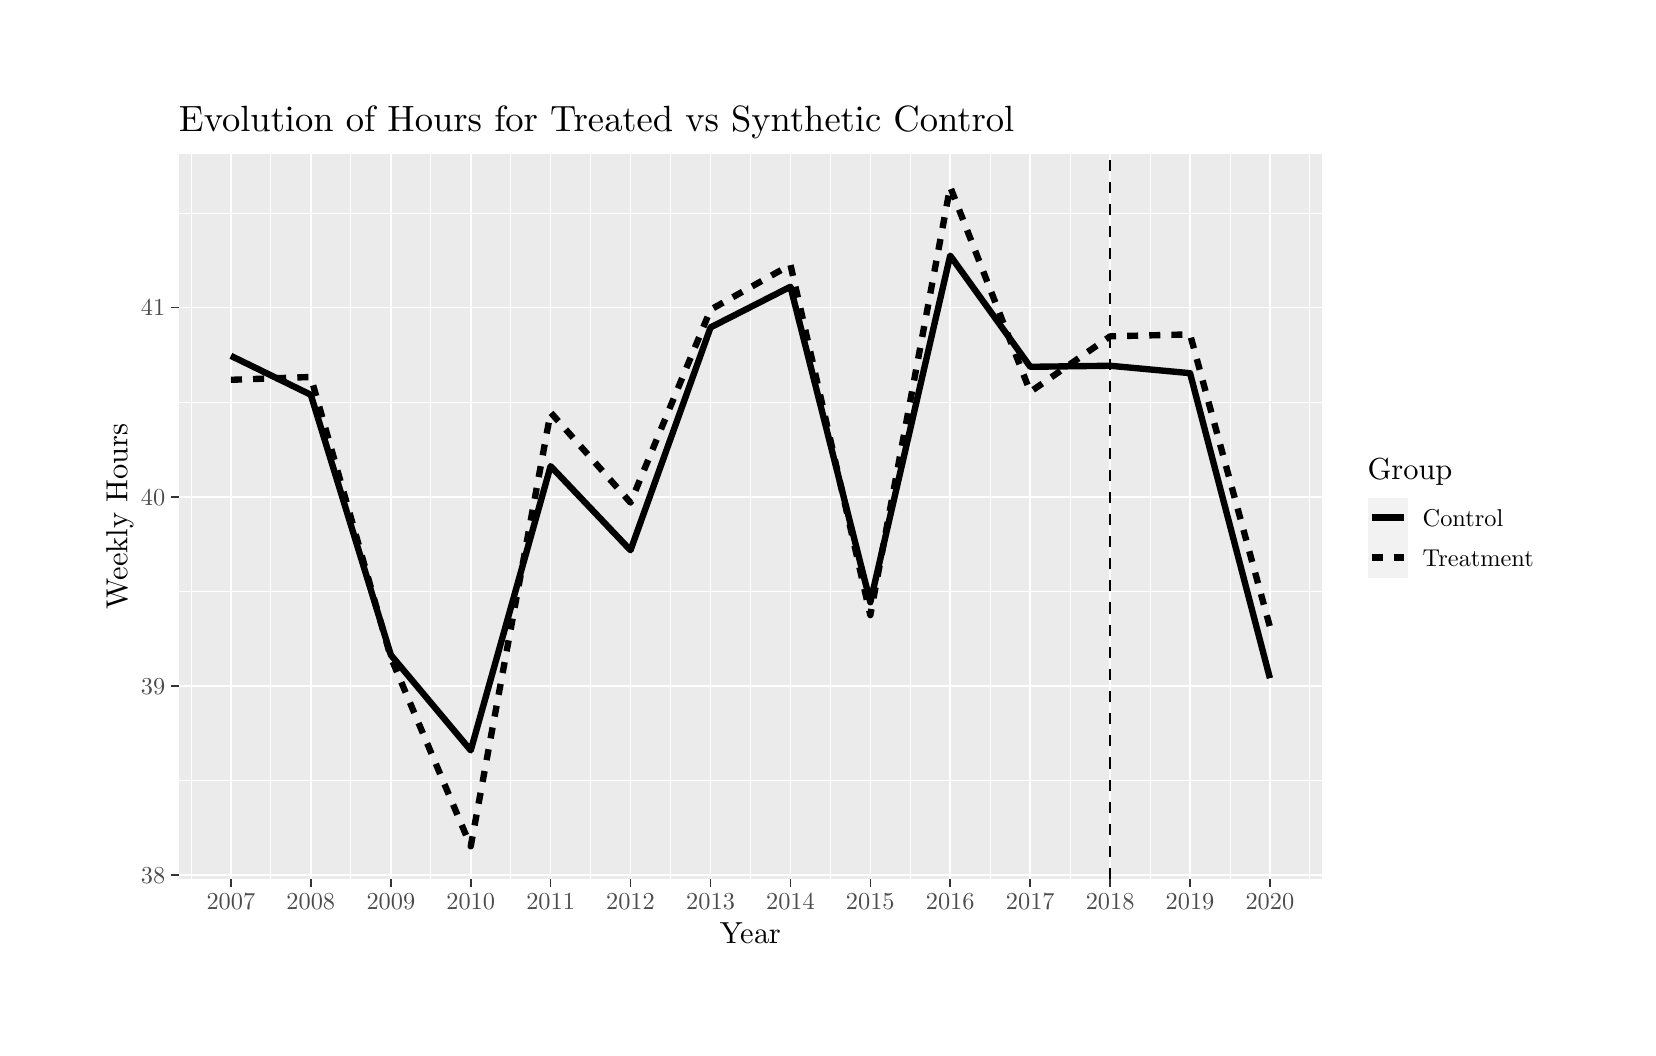
\begin{tikzpicture}[x=1pt,y=1pt]
\definecolor{fillColor}{RGB}{255,255,255}
\path[use as bounding box,fill=fillColor,fill opacity=0.00] (0,0) rectangle (578.16,361.35);
\begin{scope}
\path[clip] (  0.00,  0.00) rectangle (578.16,361.35);
\definecolor{drawColor}{RGB}{255,255,255}
\definecolor{fillColor}{RGB}{255,255,255}

\path[draw=drawColor,line width= 0.6pt,line join=round,line cap=round,fill=fillColor] (  0.00,  0.00) rectangle (578.16,361.35);
\end{scope}
\begin{scope}
\path[clip] ( 54.66, 53.64) rectangle (467.65,315.74);
\definecolor{fillColor}{gray}{0.92}

\path[fill=fillColor] ( 54.66, 53.64) rectangle (467.65,315.74);
\definecolor{drawColor}{RGB}{255,255,255}

\path[draw=drawColor,line width= 0.3pt,line join=round] ( 54.66, 89.25) --
	(467.65, 89.25);

\path[draw=drawColor,line width= 0.3pt,line join=round] ( 54.66,157.63) --
	(467.65,157.63);

\path[draw=drawColor,line width= 0.3pt,line join=round] ( 54.66,226.01) --
	(467.65,226.01);

\path[draw=drawColor,line width= 0.3pt,line join=round] ( 54.66,294.39) --
	(467.65,294.39);

\path[draw=drawColor,line width= 0.3pt,line join=round] ( 59.01, 53.64) --
	( 59.01,315.74);

\path[draw=drawColor,line width= 0.3pt,line join=round] ( 87.87, 53.64) --
	( 87.87,315.74);

\path[draw=drawColor,line width= 0.3pt,line join=round] (116.77, 53.64) --
	(116.77,315.74);

\path[draw=drawColor,line width= 0.3pt,line join=round] (145.67, 53.64) --
	(145.67,315.74);

\path[draw=drawColor,line width= 0.3pt,line join=round] (174.53, 53.64) --
	(174.53,315.74);

\path[draw=drawColor,line width= 0.3pt,line join=round] (203.39, 53.64) --
	(203.39,315.74);

\path[draw=drawColor,line width= 0.3pt,line join=round] (232.30, 53.64) --
	(232.30,315.74);

\path[draw=drawColor,line width= 0.3pt,line join=round] (261.20, 53.64) --
	(261.20,315.74);

\path[draw=drawColor,line width= 0.3pt,line join=round] (290.06, 53.64) --
	(290.06,315.74);

\path[draw=drawColor,line width= 0.3pt,line join=round] (318.92, 53.64) --
	(318.92,315.74);

\path[draw=drawColor,line width= 0.3pt,line join=round] (347.82, 53.64) --
	(347.82,315.74);

\path[draw=drawColor,line width= 0.3pt,line join=round] (376.72, 53.64) --
	(376.72,315.74);

\path[draw=drawColor,line width= 0.3pt,line join=round] (405.58, 53.64) --
	(405.58,315.74);

\path[draw=drawColor,line width= 0.3pt,line join=round] (434.45, 53.64) --
	(434.45,315.74);

\path[draw=drawColor,line width= 0.3pt,line join=round] (463.31, 53.64) --
	(463.31,315.74);

\path[draw=drawColor,line width= 0.6pt,line join=round] ( 54.66, 55.05) --
	(467.65, 55.05);

\path[draw=drawColor,line width= 0.6pt,line join=round] ( 54.66,123.44) --
	(467.65,123.44);

\path[draw=drawColor,line width= 0.6pt,line join=round] ( 54.66,191.82) --
	(467.65,191.82);

\path[draw=drawColor,line width= 0.6pt,line join=round] ( 54.66,260.20) --
	(467.65,260.20);

\path[draw=drawColor,line width= 0.6pt,line join=round] ( 73.44, 53.64) --
	( 73.44,315.74);

\path[draw=drawColor,line width= 0.6pt,line join=round] (102.30, 53.64) --
	(102.30,315.74);

\path[draw=drawColor,line width= 0.6pt,line join=round] (131.24, 53.64) --
	(131.24,315.74);

\path[draw=drawColor,line width= 0.6pt,line join=round] (160.10, 53.64) --
	(160.10,315.74);

\path[draw=drawColor,line width= 0.6pt,line join=round] (188.96, 53.64) --
	(188.96,315.74);

\path[draw=drawColor,line width= 0.6pt,line join=round] (217.83, 53.64) --
	(217.83,315.74);

\path[draw=drawColor,line width= 0.6pt,line join=round] (246.77, 53.64) --
	(246.77,315.74);

\path[draw=drawColor,line width= 0.6pt,line join=round] (275.63, 53.64) --
	(275.63,315.74);

\path[draw=drawColor,line width= 0.6pt,line join=round] (304.49, 53.64) --
	(304.49,315.74);

\path[draw=drawColor,line width= 0.6pt,line join=round] (333.35, 53.64) --
	(333.35,315.74);

\path[draw=drawColor,line width= 0.6pt,line join=round] (362.29, 53.64) --
	(362.29,315.74);

\path[draw=drawColor,line width= 0.6pt,line join=round] (391.15, 53.64) --
	(391.15,315.74);

\path[draw=drawColor,line width= 0.6pt,line join=round] (420.02, 53.64) --
	(420.02,315.74);

\path[draw=drawColor,line width= 0.6pt,line join=round] (448.88, 53.64) --
	(448.88,315.74);
\definecolor{drawColor}{RGB}{0,0,0}

\path[draw=drawColor,line width= 2.3pt,dash pattern=on 4pt off 4pt ,line join=round] ( 73.44,234.10) --
	(102.30,235.12) --
	(131.24,133.73) --
	(160.10, 65.55) --
	(188.96,222.32) --
	(217.83,189.72) --
	(246.77,259.46) --
	(275.63,275.65) --
	(304.49,149.06) --
	(333.35,303.83) --
	(362.29,229.74) --
	(391.15,249.81) --
	(420.02,250.52) --
	(448.88,144.86);

\path[draw=drawColor,line width= 2.3pt,line join=round] ( 73.44,242.76) --
	(102.30,228.71) --
	(131.24,134.66) --
	(160.10,100.19) --
	(188.96,202.91) --
	(217.83,172.51) --
	(246.77,253.05) --
	(275.63,267.74) --
	(304.49,153.73) --
	(333.35,278.99) --
	(362.29,238.80) --
	(391.15,239.18) --
	(420.02,236.50) --
	(448.88,126.28);

\path[draw=drawColor,line width= 0.6pt,dash pattern=on 4pt off 4pt ,line join=round] (391.15, 53.64) -- (391.15,315.74);
\end{scope}
\begin{scope}
\path[clip] (  0.00,  0.00) rectangle (578.16,361.35);
\definecolor{drawColor}{gray}{0.30}

\node[text=drawColor,anchor=base east,inner sep=0pt, outer sep=0pt, scale=  0.88] at ( 49.71, 52.02) {38};

\node[text=drawColor,anchor=base east,inner sep=0pt, outer sep=0pt, scale=  0.88] at ( 49.71,120.41) {39};

\node[text=drawColor,anchor=base east,inner sep=0pt, outer sep=0pt, scale=  0.88] at ( 49.71,188.79) {40};

\node[text=drawColor,anchor=base east,inner sep=0pt, outer sep=0pt, scale=  0.88] at ( 49.71,257.17) {41};
\end{scope}
\begin{scope}
\path[clip] (  0.00,  0.00) rectangle (578.16,361.35);
\definecolor{drawColor}{gray}{0.20}

\path[draw=drawColor,line width= 0.6pt,line join=round] ( 51.91, 55.05) --
	( 54.66, 55.05);

\path[draw=drawColor,line width= 0.6pt,line join=round] ( 51.91,123.44) --
	( 54.66,123.44);

\path[draw=drawColor,line width= 0.6pt,line join=round] ( 51.91,191.82) --
	( 54.66,191.82);

\path[draw=drawColor,line width= 0.6pt,line join=round] ( 51.91,260.20) --
	( 54.66,260.20);
\end{scope}
\begin{scope}
\path[clip] (  0.00,  0.00) rectangle (578.16,361.35);
\definecolor{drawColor}{gray}{0.20}

\path[draw=drawColor,line width= 0.6pt,line join=round] ( 73.44, 50.89) --
	( 73.44, 53.64);

\path[draw=drawColor,line width= 0.6pt,line join=round] (102.30, 50.89) --
	(102.30, 53.64);

\path[draw=drawColor,line width= 0.6pt,line join=round] (131.24, 50.89) --
	(131.24, 53.64);

\path[draw=drawColor,line width= 0.6pt,line join=round] (160.10, 50.89) --
	(160.10, 53.64);

\path[draw=drawColor,line width= 0.6pt,line join=round] (188.96, 50.89) --
	(188.96, 53.64);

\path[draw=drawColor,line width= 0.6pt,line join=round] (217.83, 50.89) --
	(217.83, 53.64);

\path[draw=drawColor,line width= 0.6pt,line join=round] (246.77, 50.89) --
	(246.77, 53.64);

\path[draw=drawColor,line width= 0.6pt,line join=round] (275.63, 50.89) --
	(275.63, 53.64);

\path[draw=drawColor,line width= 0.6pt,line join=round] (304.49, 50.89) --
	(304.49, 53.64);

\path[draw=drawColor,line width= 0.6pt,line join=round] (333.35, 50.89) --
	(333.35, 53.64);

\path[draw=drawColor,line width= 0.6pt,line join=round] (362.29, 50.89) --
	(362.29, 53.64);

\path[draw=drawColor,line width= 0.6pt,line join=round] (391.15, 50.89) --
	(391.15, 53.64);

\path[draw=drawColor,line width= 0.6pt,line join=round] (420.02, 50.89) --
	(420.02, 53.64);

\path[draw=drawColor,line width= 0.6pt,line join=round] (448.88, 50.89) --
	(448.88, 53.64);
\end{scope}
\begin{scope}
\path[clip] (  0.00,  0.00) rectangle (578.16,361.35);
\definecolor{drawColor}{gray}{0.30}

\node[text=drawColor,anchor=base,inner sep=0pt, outer sep=0pt, scale=  0.88] at ( 73.44, 42.63) {2007};

\node[text=drawColor,anchor=base,inner sep=0pt, outer sep=0pt, scale=  0.88] at (102.30, 42.63) {2008};

\node[text=drawColor,anchor=base,inner sep=0pt, outer sep=0pt, scale=  0.88] at (131.24, 42.63) {2009};

\node[text=drawColor,anchor=base,inner sep=0pt, outer sep=0pt, scale=  0.88] at (160.10, 42.63) {2010};

\node[text=drawColor,anchor=base,inner sep=0pt, outer sep=0pt, scale=  0.88] at (188.96, 42.63) {2011};

\node[text=drawColor,anchor=base,inner sep=0pt, outer sep=0pt, scale=  0.88] at (217.83, 42.63) {2012};

\node[text=drawColor,anchor=base,inner sep=0pt, outer sep=0pt, scale=  0.88] at (246.77, 42.63) {2013};

\node[text=drawColor,anchor=base,inner sep=0pt, outer sep=0pt, scale=  0.88] at (275.63, 42.63) {2014};

\node[text=drawColor,anchor=base,inner sep=0pt, outer sep=0pt, scale=  0.88] at (304.49, 42.63) {2015};

\node[text=drawColor,anchor=base,inner sep=0pt, outer sep=0pt, scale=  0.88] at (333.35, 42.63) {2016};

\node[text=drawColor,anchor=base,inner sep=0pt, outer sep=0pt, scale=  0.88] at (362.29, 42.63) {2017};

\node[text=drawColor,anchor=base,inner sep=0pt, outer sep=0pt, scale=  0.88] at (391.15, 42.63) {2018};

\node[text=drawColor,anchor=base,inner sep=0pt, outer sep=0pt, scale=  0.88] at (420.02, 42.63) {2019};

\node[text=drawColor,anchor=base,inner sep=0pt, outer sep=0pt, scale=  0.88] at (448.88, 42.63) {2020};
\end{scope}
\begin{scope}
\path[clip] (  0.00,  0.00) rectangle (578.16,361.35);
\definecolor{drawColor}{RGB}{0,0,0}

\node[text=drawColor,anchor=base,inner sep=0pt, outer sep=0pt, scale=  1.10] at (261.16, 30.59) {Year};
\end{scope}
\begin{scope}
\path[clip] (  0.00,  0.00) rectangle (578.16,361.35);
\definecolor{drawColor}{RGB}{0,0,0}

\node[text=drawColor,rotate= 90.00,anchor=base,inner sep=0pt, outer sep=0pt, scale=  1.10] at ( 36.03,184.69) {Weekly Hours};
\end{scope}
\begin{scope}
\path[clip] (  0.00,  0.00) rectangle (578.16,361.35);
\definecolor{fillColor}{RGB}{255,255,255}

\path[fill=fillColor] (478.65,157.13) rectangle (549.71,212.25);
\end{scope}
\begin{scope}
\path[clip] (  0.00,  0.00) rectangle (578.16,361.35);
\definecolor{drawColor}{RGB}{0,0,0}

\node[text=drawColor,anchor=base west,inner sep=0pt, outer sep=0pt, scale=  1.10] at (484.15,198.11) {Group};
\end{scope}
\begin{scope}
\path[clip] (  0.00,  0.00) rectangle (578.16,361.35);
\definecolor{fillColor}{gray}{0.95}

\path[fill=fillColor] (484.15,177.08) rectangle (498.60,191.54);
\end{scope}
\begin{scope}
\path[clip] (  0.00,  0.00) rectangle (578.16,361.35);
\definecolor{drawColor}{RGB}{0,0,0}

\path[draw=drawColor,line width= 2.3pt,line join=round] (485.59,184.31) -- (497.16,184.31);
\end{scope}
\begin{scope}
\path[clip] (  0.00,  0.00) rectangle (578.16,361.35);
\definecolor{drawColor}{RGB}{0,0,0}

\path[draw=drawColor,line width= 2.3pt,line join=round] (485.59,184.31) -- (497.16,184.31);
\end{scope}
\begin{scope}
\path[clip] (  0.00,  0.00) rectangle (578.16,361.35);
\definecolor{fillColor}{gray}{0.95}

\path[fill=fillColor] (484.15,162.63) rectangle (498.60,177.08);
\end{scope}
\begin{scope}
\path[clip] (  0.00,  0.00) rectangle (578.16,361.35);
\definecolor{drawColor}{RGB}{0,0,0}

\path[draw=drawColor,line width= 2.3pt,dash pattern=on 4pt off 4pt ,line join=round] (485.59,169.86) -- (497.16,169.86);
\end{scope}
\begin{scope}
\path[clip] (  0.00,  0.00) rectangle (578.16,361.35);
\definecolor{drawColor}{RGB}{0,0,0}

\path[draw=drawColor,line width= 2.3pt,dash pattern=on 4pt off 4pt ,line join=round] (485.59,169.86) -- (497.16,169.86);
\end{scope}
\begin{scope}
\path[clip] (  0.00,  0.00) rectangle (578.16,361.35);
\definecolor{drawColor}{RGB}{0,0,0}

\node[text=drawColor,anchor=base west,inner sep=0pt, outer sep=0pt, scale=  0.88] at (504.10,181.28) {Control};
\end{scope}
\begin{scope}
\path[clip] (  0.00,  0.00) rectangle (578.16,361.35);
\definecolor{drawColor}{RGB}{0,0,0}

\node[text=drawColor,anchor=base west,inner sep=0pt, outer sep=0pt, scale=  0.88] at (504.10,166.82) {Treatment};
\end{scope}
\begin{scope}
\path[clip] (  0.00,  0.00) rectangle (578.16,361.35);
\definecolor{drawColor}{RGB}{0,0,0}

\node[text=drawColor,anchor=base west,inner sep=0pt, outer sep=0pt, scale=  1.32] at ( 54.66,323.81) {Evolution of Hours for Treated vs Synthetic Control};
\end{scope}
\end{tikzpicture}

            \end{adjustbox}
        \end{subfigure}
        \begin{subfigure}{0.4\linewidth}
            \begin{adjustbox}{width=\linewidth}
                % Created by tikzDevice version 0.12.3.1 on 2021-12-17 00:23:02
% !TEX encoding = UTF-8 Unicode
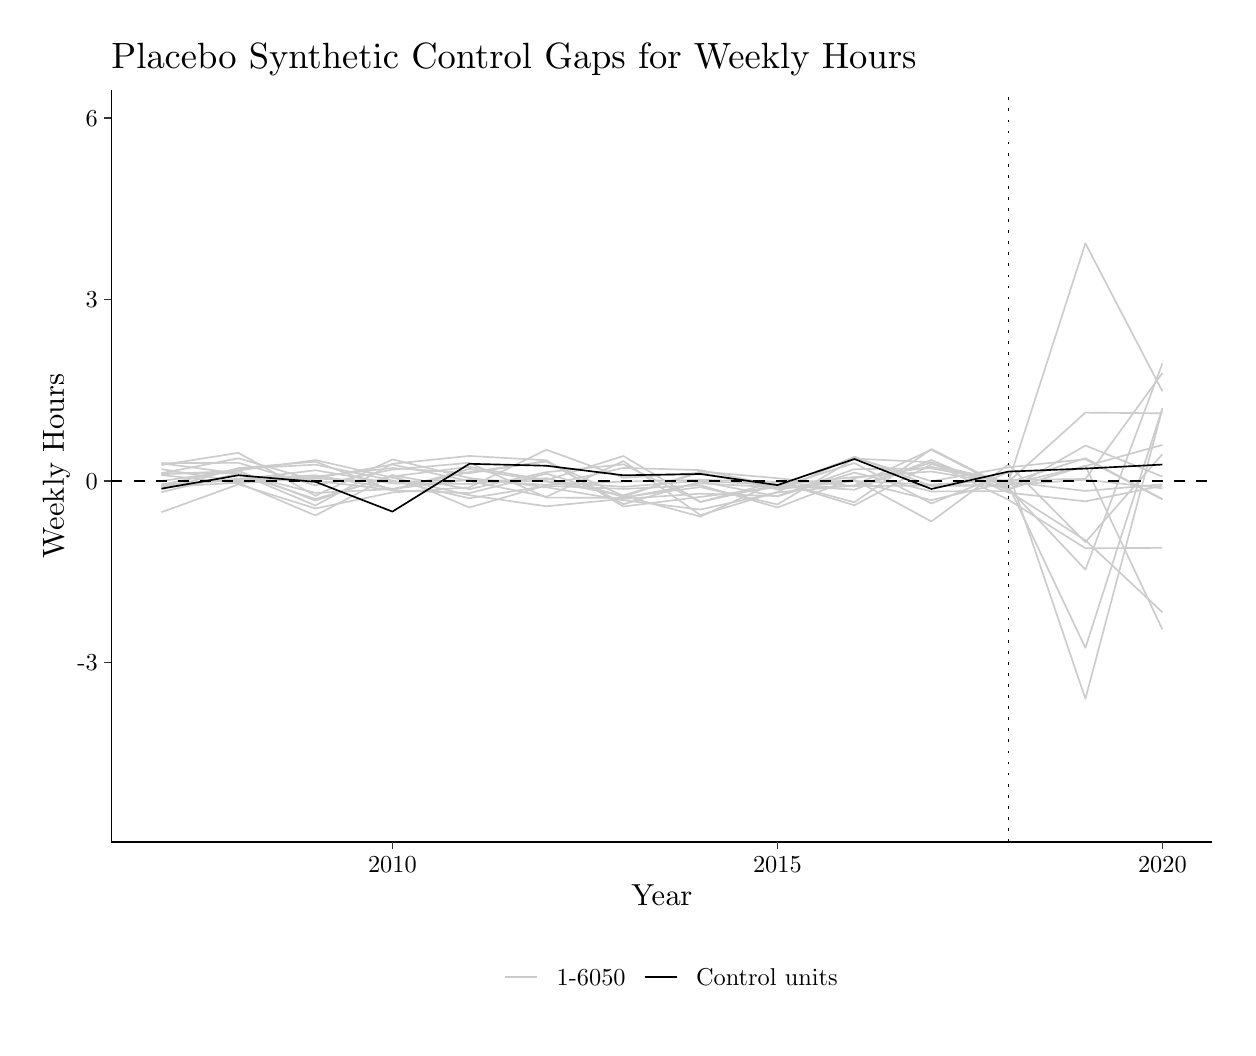
\begin{tikzpicture}[x=1pt,y=1pt]
\definecolor{fillColor}{RGB}{255,255,255}
\path[use as bounding box,fill=fillColor,fill opacity=0.00] (0,0) rectangle (433.62,361.35);
\begin{scope}
\path[clip] (  0.00,  0.00) rectangle (433.62,361.35);
\definecolor{drawColor}{RGB}{255,255,255}
\definecolor{fillColor}{RGB}{255,255,255}

\path[draw=drawColor,line width= 0.6pt,line join=round,line cap=round,fill=fillColor] (  0.00,  0.00) rectangle (433.62,361.35);
\end{scope}
\begin{scope}
\path[clip] ( 30.25, 67.14) rectangle (428.12,338.69);
\definecolor{drawColor}{gray}{0.80}

\path[draw=drawColor,line width= 0.6pt,line join=round] ( 48.33,195.41) --
	( 76.15,196.88) --
	(103.98,185.08) --
	(131.80,199.63) --
	(159.62,187.97) --
	(187.45,196.00) --
	(215.27,202.27) --
	(243.09,201.47) --
	(270.92,195.79) --
	(298.74,206.02) --
	(326.56,197.46) --
	(354.39,202.48) --
	(382.21,205.42) --
	(410.03,190.89);

\path[draw=drawColor,line width= 0.6pt,line join=round] ( 48.33,197.56) --
	( 76.15,201.34) --
	(103.98,205.10) --
	(131.80,198.75) --
	(159.62,192.40) --
	(187.45,188.40) --
	(215.27,191.09) --
	(243.09,192.96) --
	(270.92,192.08) --
	(298.74,201.82) --
	(326.56,202.10) --
	(354.39,197.04) --
	(382.21,205.77) --
	(410.03,190.98);

\path[draw=drawColor,line width= 0.6pt,line join=round] ( 48.33,200.36) --
	( 76.15,205.73) --
	(103.98,197.66) --
	(131.80,194.23) --
	(159.62,201.91) --
	(187.45,197.36) --
	(215.27,192.38) --
	(243.09,200.54) --
	(270.92,194.55) --
	(298.74,197.51) --
	(326.56,190.61) --
	(354.39,197.26) --
	(382.21,193.93) --
	(410.03,196.33);

\path[draw=drawColor,line width= 0.6pt,line join=round] ( 48.33,195.77) --
	( 76.15,198.06) --
	(103.98,201.42) --
	(131.80,196.67) --
	(159.62,196.48) --
	(187.45,198.56) --
	(215.27,191.96) --
	(243.09,200.99) --
	(270.92,198.55) --
	(298.74,195.68) --
	(326.56,195.89) --
	(354.39,196.13) --
	(382.21,198.00) --
	(410.03,194.92);

\path[draw=drawColor,line width= 0.6pt,line join=round] ( 48.33,203.92) --
	( 76.15,200.21) --
	(103.98,193.24) --
	(131.80,194.60) --
	(159.62,200.77) --
	(187.45,204.56) --
	(215.27,192.16) --
	(243.09,184.67) --
	(270.92,197.25) --
	(298.74,188.76) --
	(326.56,203.58) --
	(354.39,197.16) --
	(382.21,283.42) --
	(410.03,229.95);

\path[draw=drawColor,line width= 0.6pt,line join=round] ( 48.33,186.26) --
	( 76.15,196.33) --
	(103.98,187.62) --
	(131.80,193.41) --
	(159.62,195.25) --
	(187.45,208.83) --
	(215.27,198.73) --
	(243.09,200.43) --
	(270.92,195.16) --
	(298.74,204.02) --
	(326.56,189.40) --
	(354.39,200.76) --
	(382.21,118.84) --
	(410.03,223.63);

\path[draw=drawColor,line width= 0.6pt,line join=round] ( 48.33,203.31) --
	( 76.15,207.71) --
	(103.98,192.19) --
	(131.80,205.34) --
	(159.62,198.61) --
	(187.45,195.28) --
	(215.27,190.58) --
	(243.09,187.22) --
	(270.92,193.41) --
	(298.74,196.00) --
	(326.56,208.83) --
	(354.39,194.55) --
	(382.21,203.02) --
	(410.03,143.87);

\path[draw=drawColor,line width= 0.6pt,line join=round] ( 48.33,195.63) --
	( 76.15,198.39) --
	(103.98,199.59) --
	(131.80,194.72) --
	(159.62,197.97) --
	(187.45,197.36) --
	(215.27,195.43) --
	(243.09,197.62) --
	(270.92,195.99) --
	(298.74,198.96) --
	(326.56,200.96) --
	(354.39,196.34) --
	(382.21,202.90) --
	(410.03,210.56);

\path[draw=drawColor,line width= 0.6pt,line join=round] ( 48.33,200.33) --
	( 76.15,200.36) --
	(103.98,188.67) --
	(131.80,203.76) --
	(159.62,206.59) --
	(187.45,205.03) --
	(215.27,188.31) --
	(243.09,191.80) --
	(270.92,195.29) --
	(298.74,195.62) --
	(326.56,204.20) --
	(354.39,190.76) --
	(382.21,173.22) --
	(410.03,173.38);

\path[draw=drawColor,line width= 0.6pt,line join=round] ( 48.33,196.34) --
	( 76.15,197.91) --
	(103.98,198.43) --
	(131.80,197.26) --
	(159.62,197.85) --
	(187.45,196.16) --
	(215.27,197.32) --
	(243.09,197.98) --
	(270.92,197.24) --
	(298.74,197.50) --
	(326.56,196.28) --
	(354.39,197.89) --
	(382.21,198.28) --
	(410.03,236.56);

\path[draw=drawColor,line width= 0.6pt,line join=round] ( 48.33,196.18) --
	( 76.15,201.96) --
	(103.98,203.44) --
	(131.80,197.74) --
	(159.62,191.28) --
	(187.45,195.79) --
	(215.27,194.67) --
	(243.09,195.98) --
	(270.92,187.96) --
	(298.74,198.57) --
	(326.56,202.62) --
	(354.39,197.23) --
	(382.21,222.24) --
	(410.03,222.01);

\path[draw=drawColor,line width= 0.6pt,line join=round] ( 48.33,193.48) --
	( 76.15,200.25) --
	(103.98,191.02) --
	(131.80,199.19) --
	(159.62,202.65) --
	(187.45,197.84) --
	(215.27,206.56) --
	(243.09,189.98) --
	(270.92,197.30) --
	(298.74,189.85) --
	(326.56,209.08) --
	(354.39,195.01) --
	(382.21,165.50) --
	(410.03,240.05);

\path[draw=drawColor,line width= 0.6pt,line join=round] ( 48.33,203.98) --
	( 76.15,204.10) --
	(103.98,195.98) --
	(131.80,201.67) --
	(159.62,204.11) --
	(187.45,191.55) --
	(215.27,191.41) --
	(243.09,196.71) --
	(270.92,195.22) --
	(298.74,197.99) --
	(326.56,182.92) --
	(354.39,203.50) --
	(382.21,175.44) --
	(410.03,207.22);

\path[draw=drawColor,line width= 0.6pt,line join=round] ( 48.33,199.68) --
	( 76.15,196.75) --
	(103.98,198.56) --
	(131.80,203.50) --
	(159.62,197.49) --
	(187.45,191.84) --
	(215.27,204.72) --
	(243.09,185.21) --
	(270.92,193.59) --
	(298.74,206.33) --
	(326.56,195.70) --
	(354.39,196.01) --
	(382.21,137.25) --
	(410.03,223.84);

\path[draw=drawColor,line width= 0.6pt,line join=round] ( 48.33,201.82) --
	( 76.15,197.29) --
	(103.98,199.11) --
	(131.80,202.22) --
	(159.62,200.36) --
	(187.45,204.77) --
	(215.27,189.13) --
	(243.09,197.35) --
	(270.92,191.94) --
	(298.74,200.56) --
	(326.56,193.76) --
	(354.39,193.91) --
	(382.21,176.10) --
	(410.03,150.11);

\path[draw=drawColor,line width= 0.6pt,line join=round] ( 48.33,199.96) --
	( 76.15,201.21) --
	(103.98,190.45) --
	(131.80,199.66) --
	(159.62,194.60) --
	(187.45,200.74) --
	(215.27,203.56) --
	(243.09,189.97) --
	(270.92,196.15) --
	(298.74,194.39) --
	(326.56,205.12) --
	(354.39,193.35) --
	(382.21,190.18) --
	(410.03,195.83);

\path[draw=drawColor,line width= 0.6pt,line join=round] ( 48.33,194.42) --
	( 76.15,202.22) --
	(103.98,204.52) --
	(131.80,194.16) --
	(159.62,193.15) --
	(187.45,200.19) --
	(215.27,191.74) --
	(243.09,195.33) --
	(270.92,189.07) --
	(298.74,205.63) --
	(326.56,204.31) --
	(354.39,194.33) --
	(382.21,210.36) --
	(410.03,199.13);
\definecolor{drawColor}{RGB}{0,0,0}

\path[draw=drawColor,line width= 0.6pt,dash pattern=on 1pt off 3pt ,line join=round] (354.39, 67.14) -- (354.39,338.69);

\path[draw=drawColor,line width= 0.6pt,dash pattern=on 4pt off 4pt ,line join=round] ( 30.25,197.55) -- (428.12,197.55);

\path[draw=drawColor,line width= 0.6pt,line join=round] ( 48.33,194.78) --
	( 76.15,199.60) --
	(103.98,197.25) --
	(131.80,186.48) --
	(159.62,203.75) --
	(187.45,203.05) --
	(215.27,199.60) --
	(243.09,200.07) --
	(270.92,196.05) --
	(298.74,205.48) --
	(326.56,194.65) --
	(354.39,200.94) --
	(382.21,202.03) --
	(410.03,203.48);
\end{scope}
\begin{scope}
\path[clip] (  0.00,  0.00) rectangle (433.62,361.35);
\definecolor{drawColor}{RGB}{0,0,0}

\path[draw=drawColor,line width= 0.6pt,line join=round] ( 30.25, 67.14) --
	( 30.25,338.69);
\end{scope}
\begin{scope}
\path[clip] (  0.00,  0.00) rectangle (433.62,361.35);
\definecolor{drawColor}{RGB}{0,0,0}

\node[text=drawColor,anchor=base east,inner sep=0pt, outer sep=0pt, scale=  0.88] at ( 25.30,128.98) {-3};

\node[text=drawColor,anchor=base east,inner sep=0pt, outer sep=0pt, scale=  0.88] at ( 25.30,194.52) {0};

\node[text=drawColor,anchor=base east,inner sep=0pt, outer sep=0pt, scale=  0.88] at ( 25.30,260.06) {3};

\node[text=drawColor,anchor=base east,inner sep=0pt, outer sep=0pt, scale=  0.88] at ( 25.30,325.59) {6};
\end{scope}
\begin{scope}
\path[clip] (  0.00,  0.00) rectangle (433.62,361.35);
\definecolor{drawColor}{gray}{0.20}

\path[draw=drawColor,line width= 0.6pt,line join=round] ( 27.50,132.01) --
	( 30.25,132.01);

\path[draw=drawColor,line width= 0.6pt,line join=round] ( 27.50,197.55) --
	( 30.25,197.55);

\path[draw=drawColor,line width= 0.6pt,line join=round] ( 27.50,263.09) --
	( 30.25,263.09);

\path[draw=drawColor,line width= 0.6pt,line join=round] ( 27.50,328.63) --
	( 30.25,328.63);
\end{scope}
\begin{scope}
\path[clip] (  0.00,  0.00) rectangle (433.62,361.35);
\definecolor{drawColor}{RGB}{0,0,0}

\path[draw=drawColor,line width= 0.6pt,line join=round] ( 30.25, 67.14) --
	(428.12, 67.14);
\end{scope}
\begin{scope}
\path[clip] (  0.00,  0.00) rectangle (433.62,361.35);
\definecolor{drawColor}{gray}{0.20}

\path[draw=drawColor,line width= 0.6pt,line join=round] (131.80, 64.39) --
	(131.80, 67.14);

\path[draw=drawColor,line width= 0.6pt,line join=round] (270.92, 64.39) --
	(270.92, 67.14);

\path[draw=drawColor,line width= 0.6pt,line join=round] (410.03, 64.39) --
	(410.03, 67.14);
\end{scope}
\begin{scope}
\path[clip] (  0.00,  0.00) rectangle (433.62,361.35);
\definecolor{drawColor}{RGB}{0,0,0}

\node[text=drawColor,anchor=base,inner sep=0pt, outer sep=0pt, scale=  0.88] at (131.80, 56.13) {2010};

\node[text=drawColor,anchor=base,inner sep=0pt, outer sep=0pt, scale=  0.88] at (270.92, 56.13) {2015};

\node[text=drawColor,anchor=base,inner sep=0pt, outer sep=0pt, scale=  0.88] at (410.03, 56.13) {2020};
\end{scope}
\begin{scope}
\path[clip] (  0.00,  0.00) rectangle (433.62,361.35);
\definecolor{drawColor}{RGB}{0,0,0}

\node[text=drawColor,anchor=base,inner sep=0pt, outer sep=0pt, scale=  1.10] at (229.18, 44.09) {Year};
\end{scope}
\begin{scope}
\path[clip] (  0.00,  0.00) rectangle (433.62,361.35);
\definecolor{drawColor}{RGB}{0,0,0}

\node[text=drawColor,rotate= 90.00,anchor=base,inner sep=0pt, outer sep=0pt, scale=  1.10] at ( 13.08,202.92) {Weekly Hours};
\end{scope}
\begin{scope}
\path[clip] (  0.00,  0.00) rectangle (433.62,361.35);
\definecolor{fillColor}{RGB}{255,255,255}

\path[fill=fillColor] (160.19,  5.50) rectangle (298.18, 30.95);
\end{scope}
\begin{scope}
\path[clip] (  0.00,  0.00) rectangle (433.62,361.35);
\definecolor{drawColor}{gray}{0.80}

\path[draw=drawColor,line width= 0.6pt,line join=round] (172.64, 18.23) -- (184.20, 18.23);
\end{scope}
\begin{scope}
\path[clip] (  0.00,  0.00) rectangle (433.62,361.35);
\definecolor{drawColor}{gray}{0.80}

\path[draw=drawColor,line width= 0.6pt,line join=round] (172.64, 18.23) -- (184.20, 18.23);
\end{scope}
\begin{scope}
\path[clip] (  0.00,  0.00) rectangle (433.62,361.35);
\definecolor{drawColor}{RGB}{0,0,0}

\path[draw=drawColor,line width= 0.6pt,line join=round] (223.02, 18.23) -- (234.58, 18.23);
\end{scope}
\begin{scope}
\path[clip] (  0.00,  0.00) rectangle (433.62,361.35);
\definecolor{drawColor}{RGB}{0,0,0}

\path[draw=drawColor,line width= 0.6pt,line join=round] (223.02, 18.23) -- (234.58, 18.23);
\end{scope}
\begin{scope}
\path[clip] (  0.00,  0.00) rectangle (433.62,361.35);
\definecolor{drawColor}{RGB}{0,0,0}

\node[text=drawColor,anchor=base west,inner sep=0pt, outer sep=0pt, scale=  0.88] at (191.14, 15.20) {1-6050};
\end{scope}
\begin{scope}
\path[clip] (  0.00,  0.00) rectangle (433.62,361.35);
\definecolor{drawColor}{RGB}{0,0,0}

\node[text=drawColor,anchor=base west,inner sep=0pt, outer sep=0pt, scale=  0.88] at (241.53, 15.20) {Control units};
\end{scope}
\begin{scope}
\path[clip] (  0.00,  0.00) rectangle (433.62,361.35);
\definecolor{drawColor}{RGB}{0,0,0}

\node[text=drawColor,anchor=base west,inner sep=0pt, outer sep=0pt, scale=  1.32] at ( 30.25,346.76) {Placebo Synthetic Control Gaps for Weekly Hours};
\end{scope}
\end{tikzpicture}

            \end{adjustbox}
        \end{subfigure}
        \begin{subfigure}{0.55\linewidth}
            \begin{adjustbox}{width=\linewidth}
                % Created by tikzDevice version 0.12.3.1 on 2021-12-16 22:51:20
% !TEX encoding = UTF-8 Unicode
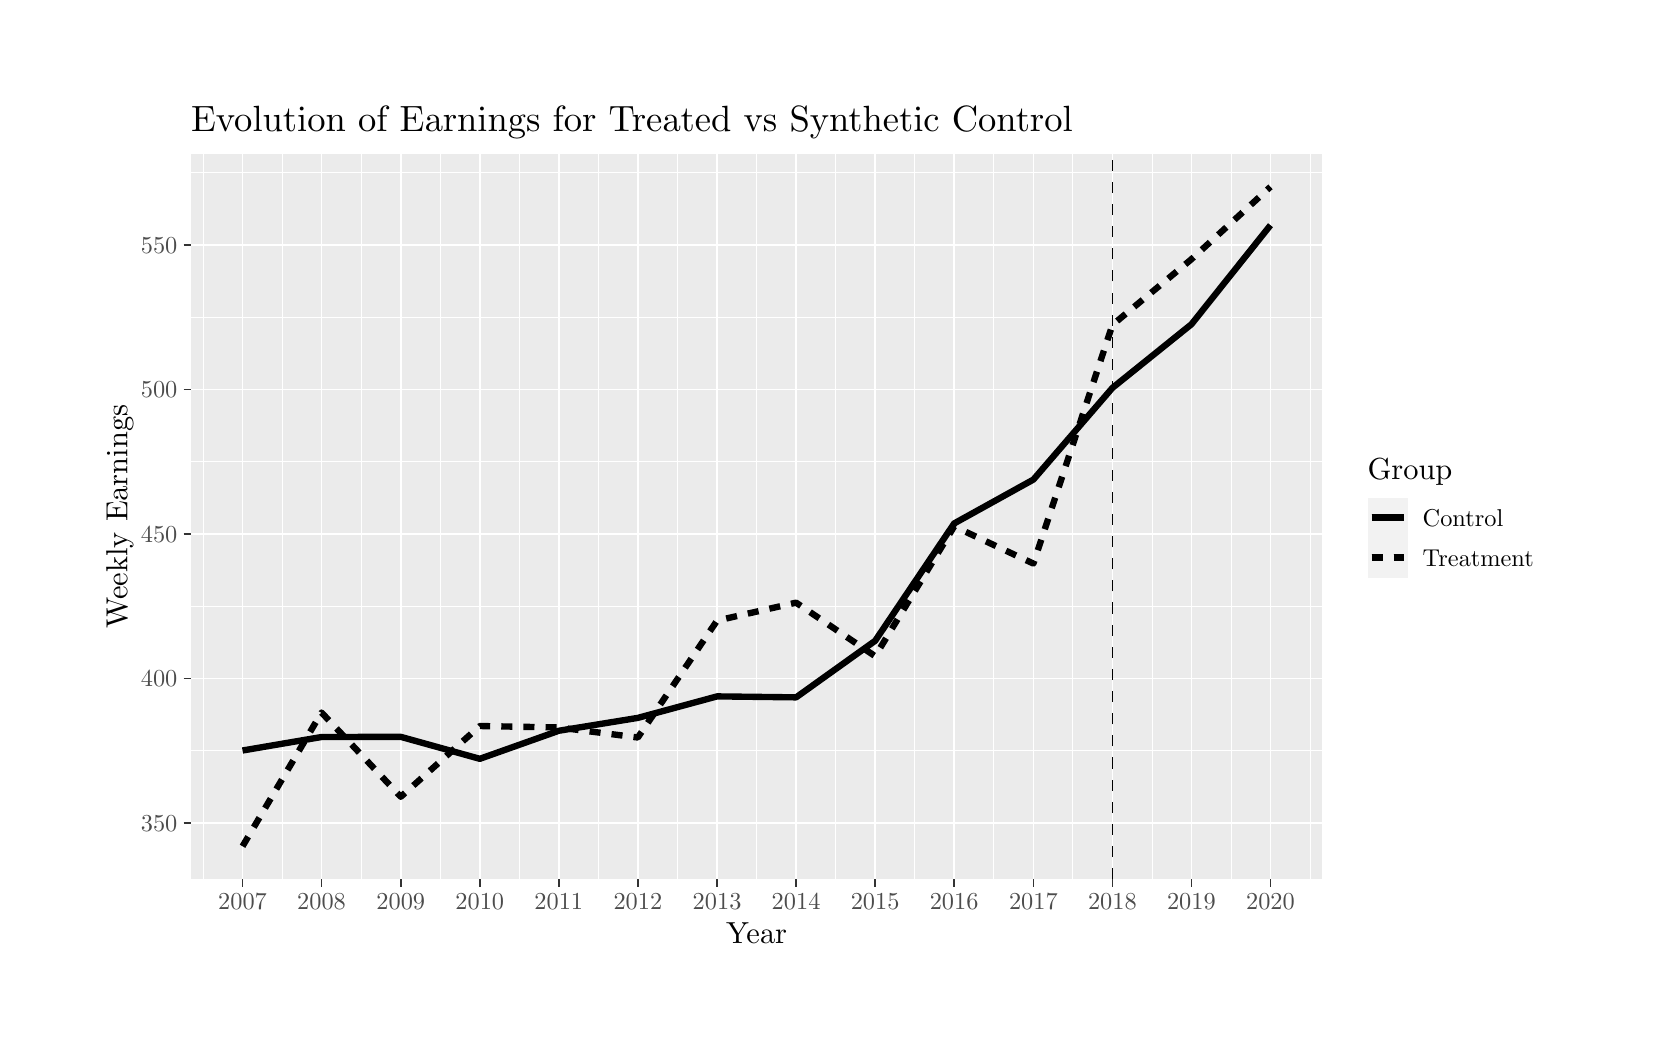
\begin{tikzpicture}[x=1pt,y=1pt]
\definecolor{fillColor}{RGB}{255,255,255}
\path[use as bounding box,fill=fillColor,fill opacity=0.00] (0,0) rectangle (578.16,361.35);
\begin{scope}
\path[clip] (  0.00,  0.00) rectangle (578.16,361.35);
\definecolor{drawColor}{RGB}{255,255,255}
\definecolor{fillColor}{RGB}{255,255,255}

\path[draw=drawColor,line width= 0.6pt,line join=round,line cap=round,fill=fillColor] (  0.00,  0.00) rectangle (578.16,361.35);
\end{scope}
\begin{scope}
\path[clip] ( 59.06, 53.64) rectangle (467.65,315.74);
\definecolor{fillColor}{gray}{0.92}

\path[fill=fillColor] ( 59.06, 53.64) rectangle (467.65,315.74);
\definecolor{drawColor}{RGB}{255,255,255}

\path[draw=drawColor,line width= 0.3pt,line join=round] ( 59.06,100.06) --
	(467.65,100.06);

\path[draw=drawColor,line width= 0.3pt,line join=round] ( 59.06,152.29) --
	(467.65,152.29);

\path[draw=drawColor,line width= 0.3pt,line join=round] ( 59.06,204.53) --
	(467.65,204.53);

\path[draw=drawColor,line width= 0.3pt,line join=round] ( 59.06,256.76) --
	(467.65,256.76);

\path[draw=drawColor,line width= 0.3pt,line join=round] ( 59.06,309.00) --
	(467.65,309.00);

\path[draw=drawColor,line width= 0.3pt,line join=round] ( 63.36, 53.64) --
	( 63.36,315.74);

\path[draw=drawColor,line width= 0.3pt,line join=round] ( 91.91, 53.64) --
	( 91.91,315.74);

\path[draw=drawColor,line width= 0.3pt,line join=round] (120.51, 53.64) --
	(120.51,315.74);

\path[draw=drawColor,line width= 0.3pt,line join=round] (149.10, 53.64) --
	(149.10,315.74);

\path[draw=drawColor,line width= 0.3pt,line join=round] (177.65, 53.64) --
	(177.65,315.74);

\path[draw=drawColor,line width= 0.3pt,line join=round] (206.21, 53.64) --
	(206.21,315.74);

\path[draw=drawColor,line width= 0.3pt,line join=round] (234.80, 53.64) --
	(234.80,315.74);

\path[draw=drawColor,line width= 0.3pt,line join=round] (263.40, 53.64) --
	(263.40,315.74);

\path[draw=drawColor,line width= 0.3pt,line join=round] (291.95, 53.64) --
	(291.95,315.74);

\path[draw=drawColor,line width= 0.3pt,line join=round] (320.50, 53.64) --
	(320.50,315.74);

\path[draw=drawColor,line width= 0.3pt,line join=round] (349.10, 53.64) --
	(349.10,315.74);

\path[draw=drawColor,line width= 0.3pt,line join=round] (377.69, 53.64) --
	(377.69,315.74);

\path[draw=drawColor,line width= 0.3pt,line join=round] (406.25, 53.64) --
	(406.25,315.74);

\path[draw=drawColor,line width= 0.3pt,line join=round] (434.80, 53.64) --
	(434.80,315.74);

\path[draw=drawColor,line width= 0.3pt,line join=round] (463.35, 53.64) --
	(463.35,315.74);

\path[draw=drawColor,line width= 0.6pt,line join=round] ( 59.06, 73.94) --
	(467.65, 73.94);

\path[draw=drawColor,line width= 0.6pt,line join=round] ( 59.06,126.18) --
	(467.65,126.18);

\path[draw=drawColor,line width= 0.6pt,line join=round] ( 59.06,178.41) --
	(467.65,178.41);

\path[draw=drawColor,line width= 0.6pt,line join=round] ( 59.06,230.65) --
	(467.65,230.65);

\path[draw=drawColor,line width= 0.6pt,line join=round] ( 59.06,282.88) --
	(467.65,282.88);

\path[draw=drawColor,line width= 0.6pt,line join=round] ( 77.64, 53.64) --
	( 77.64,315.74);

\path[draw=drawColor,line width= 0.6pt,line join=round] (106.19, 53.64) --
	(106.19,315.74);

\path[draw=drawColor,line width= 0.6pt,line join=round] (134.82, 53.64) --
	(134.82,315.74);

\path[draw=drawColor,line width= 0.6pt,line join=round] (163.38, 53.64) --
	(163.38,315.74);

\path[draw=drawColor,line width= 0.6pt,line join=round] (191.93, 53.64) --
	(191.93,315.74);

\path[draw=drawColor,line width= 0.6pt,line join=round] (220.49, 53.64) --
	(220.49,315.74);

\path[draw=drawColor,line width= 0.6pt,line join=round] (249.12, 53.64) --
	(249.12,315.74);

\path[draw=drawColor,line width= 0.6pt,line join=round] (277.67, 53.64) --
	(277.67,315.74);

\path[draw=drawColor,line width= 0.6pt,line join=round] (306.23, 53.64) --
	(306.23,315.74);

\path[draw=drawColor,line width= 0.6pt,line join=round] (334.78, 53.64) --
	(334.78,315.74);

\path[draw=drawColor,line width= 0.6pt,line join=round] (363.41, 53.64) --
	(363.41,315.74);

\path[draw=drawColor,line width= 0.6pt,line join=round] (391.97, 53.64) --
	(391.97,315.74);

\path[draw=drawColor,line width= 0.6pt,line join=round] (420.52, 53.64) --
	(420.52,315.74);

\path[draw=drawColor,line width= 0.6pt,line join=round] (449.08, 53.64) --
	(449.08,315.74);
\definecolor{drawColor}{RGB}{0,0,0}

\path[draw=drawColor,line width= 2.3pt,dash pattern=on 4pt off 4pt ,line join=round] ( 77.64, 65.55) --
	(106.19,113.87) --
	(134.82, 83.43) --
	(163.38,109.00) --
	(191.93,108.48) --
	(220.49,104.85) --
	(249.12,147.10) --
	(277.67,153.58) --
	(306.23,134.23) --
	(334.78,181.13) --
	(363.41,167.70) --
	(391.97,253.93) --
	(420.52,277.68) --
	(449.08,303.83);

\path[draw=drawColor,line width= 2.3pt,line join=round] ( 77.64,100.15) --
	(106.19,105.03) --
	(134.82,105.09) --
	(163.38, 97.15) --
	(191.93,107.29) --
	(220.49,111.94) --
	(249.12,119.71) --
	(277.67,119.36) --
	(306.23,139.79) --
	(334.78,182.20) --
	(363.41,198.05) --
	(391.97,231.19) --
	(420.52,254.17) --
	(449.08,289.97);

\path[draw=drawColor,line width= 0.6pt,dash pattern=on 4pt off 4pt ,line join=round] (391.97, 53.64) -- (391.97,315.74);
\end{scope}
\begin{scope}
\path[clip] (  0.00,  0.00) rectangle (578.16,361.35);
\definecolor{drawColor}{gray}{0.30}

\node[text=drawColor,anchor=base east,inner sep=0pt, outer sep=0pt, scale=  0.88] at ( 54.11, 70.91) {350};

\node[text=drawColor,anchor=base east,inner sep=0pt, outer sep=0pt, scale=  0.88] at ( 54.11,123.15) {400};

\node[text=drawColor,anchor=base east,inner sep=0pt, outer sep=0pt, scale=  0.88] at ( 54.11,175.38) {450};

\node[text=drawColor,anchor=base east,inner sep=0pt, outer sep=0pt, scale=  0.88] at ( 54.11,227.61) {500};

\node[text=drawColor,anchor=base east,inner sep=0pt, outer sep=0pt, scale=  0.88] at ( 54.11,279.85) {550};
\end{scope}
\begin{scope}
\path[clip] (  0.00,  0.00) rectangle (578.16,361.35);
\definecolor{drawColor}{gray}{0.20}

\path[draw=drawColor,line width= 0.6pt,line join=round] ( 56.31, 73.94) --
	( 59.06, 73.94);

\path[draw=drawColor,line width= 0.6pt,line join=round] ( 56.31,126.18) --
	( 59.06,126.18);

\path[draw=drawColor,line width= 0.6pt,line join=round] ( 56.31,178.41) --
	( 59.06,178.41);

\path[draw=drawColor,line width= 0.6pt,line join=round] ( 56.31,230.65) --
	( 59.06,230.65);

\path[draw=drawColor,line width= 0.6pt,line join=round] ( 56.31,282.88) --
	( 59.06,282.88);
\end{scope}
\begin{scope}
\path[clip] (  0.00,  0.00) rectangle (578.16,361.35);
\definecolor{drawColor}{gray}{0.20}

\path[draw=drawColor,line width= 0.6pt,line join=round] ( 77.64, 50.89) --
	( 77.64, 53.64);

\path[draw=drawColor,line width= 0.6pt,line join=round] (106.19, 50.89) --
	(106.19, 53.64);

\path[draw=drawColor,line width= 0.6pt,line join=round] (134.82, 50.89) --
	(134.82, 53.64);

\path[draw=drawColor,line width= 0.6pt,line join=round] (163.38, 50.89) --
	(163.38, 53.64);

\path[draw=drawColor,line width= 0.6pt,line join=round] (191.93, 50.89) --
	(191.93, 53.64);

\path[draw=drawColor,line width= 0.6pt,line join=round] (220.49, 50.89) --
	(220.49, 53.64);

\path[draw=drawColor,line width= 0.6pt,line join=round] (249.12, 50.89) --
	(249.12, 53.64);

\path[draw=drawColor,line width= 0.6pt,line join=round] (277.67, 50.89) --
	(277.67, 53.64);

\path[draw=drawColor,line width= 0.6pt,line join=round] (306.23, 50.89) --
	(306.23, 53.64);

\path[draw=drawColor,line width= 0.6pt,line join=round] (334.78, 50.89) --
	(334.78, 53.64);

\path[draw=drawColor,line width= 0.6pt,line join=round] (363.41, 50.89) --
	(363.41, 53.64);

\path[draw=drawColor,line width= 0.6pt,line join=round] (391.97, 50.89) --
	(391.97, 53.64);

\path[draw=drawColor,line width= 0.6pt,line join=round] (420.52, 50.89) --
	(420.52, 53.64);

\path[draw=drawColor,line width= 0.6pt,line join=round] (449.08, 50.89) --
	(449.08, 53.64);
\end{scope}
\begin{scope}
\path[clip] (  0.00,  0.00) rectangle (578.16,361.35);
\definecolor{drawColor}{gray}{0.30}

\node[text=drawColor,anchor=base,inner sep=0pt, outer sep=0pt, scale=  0.88] at ( 77.64, 42.63) {2007};

\node[text=drawColor,anchor=base,inner sep=0pt, outer sep=0pt, scale=  0.88] at (106.19, 42.63) {2008};

\node[text=drawColor,anchor=base,inner sep=0pt, outer sep=0pt, scale=  0.88] at (134.82, 42.63) {2009};

\node[text=drawColor,anchor=base,inner sep=0pt, outer sep=0pt, scale=  0.88] at (163.38, 42.63) {2010};

\node[text=drawColor,anchor=base,inner sep=0pt, outer sep=0pt, scale=  0.88] at (191.93, 42.63) {2011};

\node[text=drawColor,anchor=base,inner sep=0pt, outer sep=0pt, scale=  0.88] at (220.49, 42.63) {2012};

\node[text=drawColor,anchor=base,inner sep=0pt, outer sep=0pt, scale=  0.88] at (249.12, 42.63) {2013};

\node[text=drawColor,anchor=base,inner sep=0pt, outer sep=0pt, scale=  0.88] at (277.67, 42.63) {2014};

\node[text=drawColor,anchor=base,inner sep=0pt, outer sep=0pt, scale=  0.88] at (306.23, 42.63) {2015};

\node[text=drawColor,anchor=base,inner sep=0pt, outer sep=0pt, scale=  0.88] at (334.78, 42.63) {2016};

\node[text=drawColor,anchor=base,inner sep=0pt, outer sep=0pt, scale=  0.88] at (363.41, 42.63) {2017};

\node[text=drawColor,anchor=base,inner sep=0pt, outer sep=0pt, scale=  0.88] at (391.97, 42.63) {2018};

\node[text=drawColor,anchor=base,inner sep=0pt, outer sep=0pt, scale=  0.88] at (420.52, 42.63) {2019};

\node[text=drawColor,anchor=base,inner sep=0pt, outer sep=0pt, scale=  0.88] at (449.08, 42.63) {2020};
\end{scope}
\begin{scope}
\path[clip] (  0.00,  0.00) rectangle (578.16,361.35);
\definecolor{drawColor}{RGB}{0,0,0}

\node[text=drawColor,anchor=base,inner sep=0pt, outer sep=0pt, scale=  1.10] at (263.36, 30.59) {Year};
\end{scope}
\begin{scope}
\path[clip] (  0.00,  0.00) rectangle (578.16,361.35);
\definecolor{drawColor}{RGB}{0,0,0}

\node[text=drawColor,rotate= 90.00,anchor=base,inner sep=0pt, outer sep=0pt, scale=  1.10] at ( 36.03,184.69) {Weekly Earnings};
\end{scope}
\begin{scope}
\path[clip] (  0.00,  0.00) rectangle (578.16,361.35);
\definecolor{fillColor}{RGB}{255,255,255}

\path[fill=fillColor] (478.65,157.13) rectangle (549.71,212.25);
\end{scope}
\begin{scope}
\path[clip] (  0.00,  0.00) rectangle (578.16,361.35);
\definecolor{drawColor}{RGB}{0,0,0}

\node[text=drawColor,anchor=base west,inner sep=0pt, outer sep=0pt, scale=  1.10] at (484.15,198.11) {Group};
\end{scope}
\begin{scope}
\path[clip] (  0.00,  0.00) rectangle (578.16,361.35);
\definecolor{fillColor}{gray}{0.95}

\path[fill=fillColor] (484.15,177.08) rectangle (498.60,191.54);
\end{scope}
\begin{scope}
\path[clip] (  0.00,  0.00) rectangle (578.16,361.35);
\definecolor{drawColor}{RGB}{0,0,0}

\path[draw=drawColor,line width= 2.3pt,line join=round] (485.59,184.31) -- (497.16,184.31);
\end{scope}
\begin{scope}
\path[clip] (  0.00,  0.00) rectangle (578.16,361.35);
\definecolor{drawColor}{RGB}{0,0,0}

\path[draw=drawColor,line width= 2.3pt,line join=round] (485.59,184.31) -- (497.16,184.31);
\end{scope}
\begin{scope}
\path[clip] (  0.00,  0.00) rectangle (578.16,361.35);
\definecolor{fillColor}{gray}{0.95}

\path[fill=fillColor] (484.15,162.63) rectangle (498.60,177.08);
\end{scope}
\begin{scope}
\path[clip] (  0.00,  0.00) rectangle (578.16,361.35);
\definecolor{drawColor}{RGB}{0,0,0}

\path[draw=drawColor,line width= 2.3pt,dash pattern=on 4pt off 4pt ,line join=round] (485.59,169.86) -- (497.16,169.86);
\end{scope}
\begin{scope}
\path[clip] (  0.00,  0.00) rectangle (578.16,361.35);
\definecolor{drawColor}{RGB}{0,0,0}

\path[draw=drawColor,line width= 2.3pt,dash pattern=on 4pt off 4pt ,line join=round] (485.59,169.86) -- (497.16,169.86);
\end{scope}
\begin{scope}
\path[clip] (  0.00,  0.00) rectangle (578.16,361.35);
\definecolor{drawColor}{RGB}{0,0,0}

\node[text=drawColor,anchor=base west,inner sep=0pt, outer sep=0pt, scale=  0.88] at (504.10,181.28) {Control};
\end{scope}
\begin{scope}
\path[clip] (  0.00,  0.00) rectangle (578.16,361.35);
\definecolor{drawColor}{RGB}{0,0,0}

\node[text=drawColor,anchor=base west,inner sep=0pt, outer sep=0pt, scale=  0.88] at (504.10,166.82) {Treatment};
\end{scope}
\begin{scope}
\path[clip] (  0.00,  0.00) rectangle (578.16,361.35);
\definecolor{drawColor}{RGB}{0,0,0}

\node[text=drawColor,anchor=base west,inner sep=0pt, outer sep=0pt, scale=  1.32] at ( 59.06,323.81) {Evolution of Earnings for Treated vs Synthetic Control};
\end{scope}
\end{tikzpicture}

            \end{adjustbox}
        \end{subfigure}
        \begin{subfigure}{0.4\linewidth}
            \begin{adjustbox}{width=\linewidth}
                % Created by tikzDevice version 0.12.3.1 on 2021-12-17 00:24:29
% !TEX encoding = UTF-8 Unicode
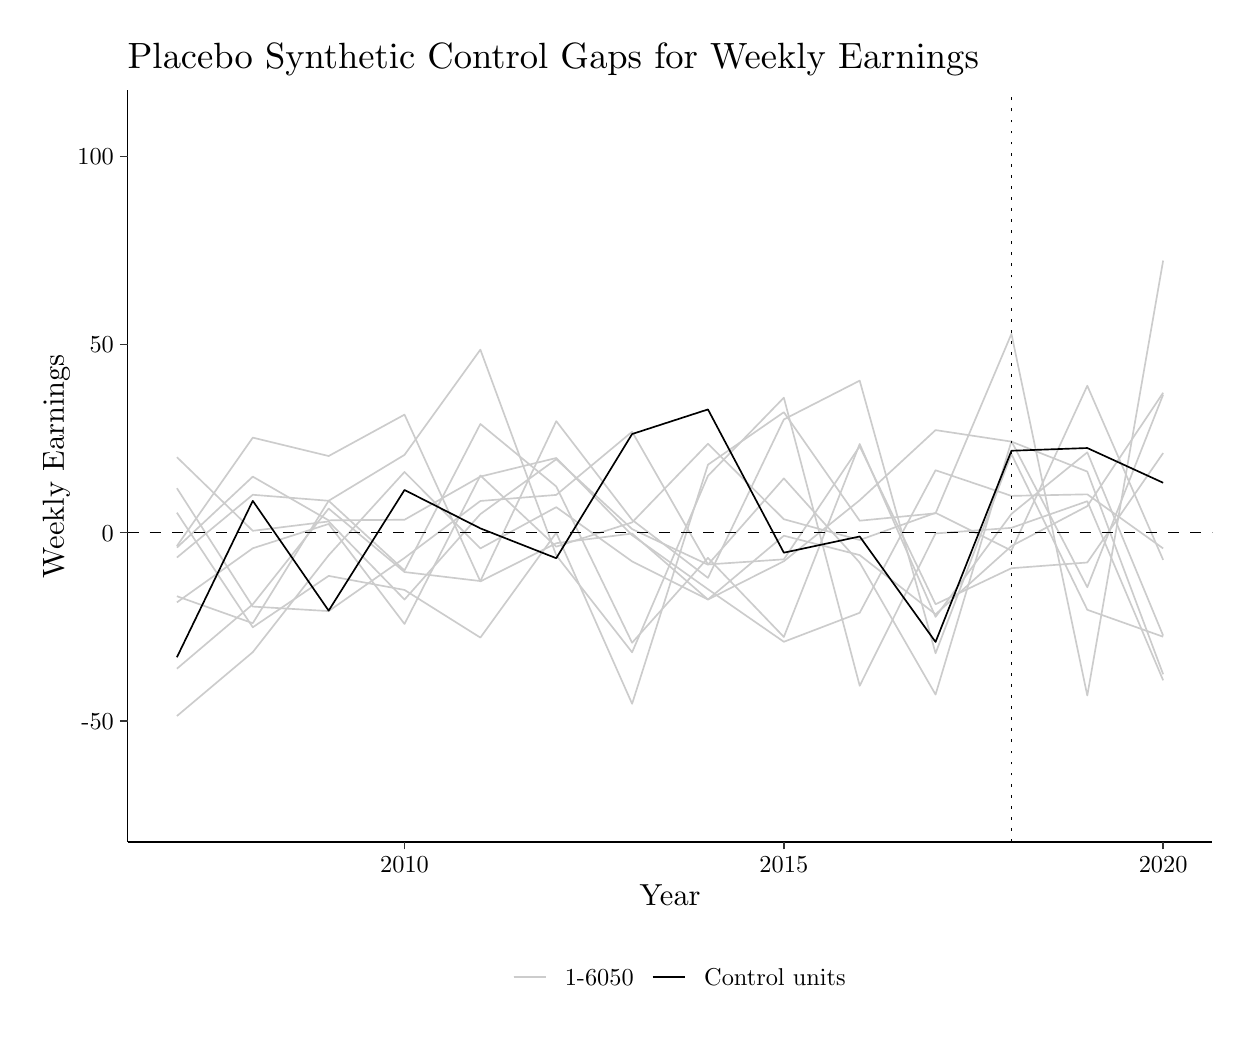
\begin{tikzpicture}[x=1pt,y=1pt]
\definecolor{fillColor}{RGB}{255,255,255}
\path[use as bounding box,fill=fillColor,fill opacity=0.00] (0,0) rectangle (433.62,361.35);
\begin{scope}
\path[clip] (  0.00,  0.00) rectangle (433.62,361.35);
\definecolor{drawColor}{RGB}{255,255,255}
\definecolor{fillColor}{RGB}{255,255,255}

\path[draw=drawColor,line width= 0.6pt,line join=round,line cap=round,fill=fillColor] (  0.00,  0.00) rectangle (433.62,361.35);
\end{scope}
\begin{scope}
\path[clip] ( 36.11, 67.14) rectangle (428.12,338.69);
\definecolor{drawColor}{gray}{0.80}

\path[draw=drawColor,line width= 0.6pt,line join=round] ( 53.93,129.72) --
	( 81.34,152.98) --
	(108.76,187.57) --
	(136.17,164.64) --
	(163.58,161.38) --
	(191.00,219.16) --
	(218.41,183.49) --
	(245.82,162.53) --
	(273.24,219.79) --
	(300.65,233.80) --
	(328.06,135.29) --
	(355.48,207.25) --
	(382.89,151.00) --
	(410.30,141.26);

\path[draw=drawColor,line width= 0.6pt,line join=round] ( 53.93,173.47) --
	( 81.34,199.11) --
	(108.76,183.32) --
	(136.17,183.54) --
	(163.58,199.13) --
	(191.00,205.85) --
	(218.41,177.94) --
	(245.82,158.43) --
	(273.24,139.44) --
	(300.65,149.92) --
	(328.06,201.43) --
	(355.48,192.16) --
	(382.89,192.72) --
	(410.30,173.17);

\path[draw=drawColor,line width= 0.6pt,line join=round] ( 53.93,174.06) --
	( 81.34,213.21) --
	(108.76,206.56) --
	(136.17,221.52) --
	(163.58,161.26) --
	(191.00,175.06) --
	(218.41,178.55) --
	(245.82,154.72) --
	(273.24,177.77) --
	(300.65,170.76) --
	(328.06,149.37) --
	(355.48,174.04) --
	(382.89,188.45) --
	(410.30,229.42);

\path[draw=drawColor,line width= 0.6pt,line join=round] ( 53.93,153.68) --
	( 81.34,173.23) --
	(108.76,182.01) --
	(136.17,145.88) --
	(163.58,199.52) --
	(191.00,173.81) --
	(218.41,182.58) --
	(245.82,210.98) --
	(273.24,183.73) --
	(300.65,176.22) --
	(328.06,186.03) --
	(355.48,172.40) --
	(382.89,231.96) --
	(410.30,169.04);

\path[draw=drawColor,line width= 0.6pt,line join=round] ( 53.93,155.90) --
	( 81.34,146.15) --
	(108.76,190.40) --
	(136.17,206.98) --
	(163.58,245.00) --
	(191.00,170.68) --
	(218.41,135.64) --
	(245.82,199.41) --
	(273.24,227.65) --
	(300.65,123.55) --
	(328.06,178.59) --
	(355.48,180.61) --
	(382.89,190.23) --
	(410.30,125.52);

\path[draw=drawColor,line width= 0.6pt,line join=round] ( 53.93,186.08) --
	( 81.34,144.68) --
	(108.76,163.25) --
	(136.17,158.17) --
	(163.58,140.95) --
	(191.00,178.82) --
	(218.41,117.03) --
	(245.82,203.43) --
	(273.24,222.40) --
	(300.65,183.19) --
	(328.06,185.86) --
	(355.48,250.71) --
	(382.89,120.02) --
	(410.30,277.19);

\path[draw=drawColor,line width= 0.6pt,line join=round] ( 53.93,206.15) --
	( 81.34,179.54) --
	(108.76,182.92) --
	(136.17,154.70) --
	(163.58,185.58) --
	(191.00,205.41) --
	(218.41,180.16) --
	(245.82,167.32) --
	(273.24,198.48) --
	(300.65,168.04) --
	(328.06,120.37) --
	(355.48,211.92) --
	(382.89,159.15) --
	(410.30,228.75);

\path[draw=drawColor,line width= 0.6pt,line join=round] ( 53.93,169.88) --
	( 81.34,192.56) --
	(108.76,190.39) --
	(136.17,165.20) --
	(163.58,218.14) --
	(191.00,195.56) --
	(218.41,139.09) --
	(245.82,169.76) --
	(273.24,141.18) --
	(300.65,210.91) --
	(328.06,148.44) --
	(355.48,185.65) --
	(382.89,207.90) --
	(410.30,141.66);

\path[draw=drawColor,line width= 0.6pt,line join=round] ( 53.93,194.93) --
	( 81.34,152.16) --
	(108.76,150.53) --
	(136.17,169.74) --
	(163.58,190.32) --
	(191.00,192.51) --
	(218.41,215.34) --
	(245.82,167.38) --
	(273.24,169.23) --
	(300.65,210.07) --
	(328.06,153.00) --
	(355.48,166.02) --
	(382.89,168.09) --
	(410.30,207.63);

\path[draw=drawColor,line width= 0.6pt,line join=round] ( 53.93,112.61) --
	( 81.34,135.69) --
	(108.76,170.70) --
	(136.17,200.81) --
	(163.58,173.17) --
	(191.00,188.08) --
	(218.41,168.48) --
	(245.82,154.71) --
	(273.24,168.54) --
	(300.65,190.58) --
	(328.06,215.93) --
	(355.48,211.77) --
	(382.89,200.94) --
	(410.30,127.70);
\definecolor{drawColor}{RGB}{0,0,0}

\path[draw=drawColor,line width= 0.6pt,dash pattern=on 1pt off 3pt ,line join=round] (355.48, 67.14) -- (355.48,338.69);

\path[draw=drawColor,line width= 0.6pt,dash pattern=on 4pt off 4pt ,line join=round] ( 36.11,178.87) -- (428.12,178.87);

\path[draw=drawColor,line width= 0.6pt,line join=round] ( 53.93,133.85) --
	( 81.34,190.37) --
	(108.76,150.69) --
	(136.17,194.29) --
	(163.58,180.42) --
	(191.00,169.64) --
	(218.41,214.51) --
	(245.82,223.40) --
	(273.24,171.63) --
	(300.65,177.49) --
	(328.06,139.38) --
	(355.48,208.47) --
	(382.89,209.45) --
	(410.30,196.90);
\end{scope}
\begin{scope}
\path[clip] (  0.00,  0.00) rectangle (433.62,361.35);
\definecolor{drawColor}{RGB}{0,0,0}

\path[draw=drawColor,line width= 0.6pt,line join=round] ( 36.11, 67.14) --
	( 36.11,338.69);
\end{scope}
\begin{scope}
\path[clip] (  0.00,  0.00) rectangle (433.62,361.35);
\definecolor{drawColor}{RGB}{0,0,0}

\node[text=drawColor,anchor=base east,inner sep=0pt, outer sep=0pt, scale=  0.88] at ( 31.16,107.87) {-50};

\node[text=drawColor,anchor=base east,inner sep=0pt, outer sep=0pt, scale=  0.88] at ( 31.16,175.84) {0};

\node[text=drawColor,anchor=base east,inner sep=0pt, outer sep=0pt, scale=  0.88] at ( 31.16,243.81) {50};

\node[text=drawColor,anchor=base east,inner sep=0pt, outer sep=0pt, scale=  0.88] at ( 31.16,311.78) {100};
\end{scope}
\begin{scope}
\path[clip] (  0.00,  0.00) rectangle (433.62,361.35);
\definecolor{drawColor}{gray}{0.20}

\path[draw=drawColor,line width= 0.6pt,line join=round] ( 33.36,110.90) --
	( 36.11,110.90);

\path[draw=drawColor,line width= 0.6pt,line join=round] ( 33.36,178.87) --
	( 36.11,178.87);

\path[draw=drawColor,line width= 0.6pt,line join=round] ( 33.36,246.84) --
	( 36.11,246.84);

\path[draw=drawColor,line width= 0.6pt,line join=round] ( 33.36,314.81) --
	( 36.11,314.81);
\end{scope}
\begin{scope}
\path[clip] (  0.00,  0.00) rectangle (433.62,361.35);
\definecolor{drawColor}{RGB}{0,0,0}

\path[draw=drawColor,line width= 0.6pt,line join=round] ( 36.11, 67.14) --
	(428.12, 67.14);
\end{scope}
\begin{scope}
\path[clip] (  0.00,  0.00) rectangle (433.62,361.35);
\definecolor{drawColor}{gray}{0.20}

\path[draw=drawColor,line width= 0.6pt,line join=round] (136.17, 64.39) --
	(136.17, 67.14);

\path[draw=drawColor,line width= 0.6pt,line join=round] (273.24, 64.39) --
	(273.24, 67.14);

\path[draw=drawColor,line width= 0.6pt,line join=round] (410.30, 64.39) --
	(410.30, 67.14);
\end{scope}
\begin{scope}
\path[clip] (  0.00,  0.00) rectangle (433.62,361.35);
\definecolor{drawColor}{RGB}{0,0,0}

\node[text=drawColor,anchor=base,inner sep=0pt, outer sep=0pt, scale=  0.88] at (136.17, 56.13) {2010};

\node[text=drawColor,anchor=base,inner sep=0pt, outer sep=0pt, scale=  0.88] at (273.24, 56.13) {2015};

\node[text=drawColor,anchor=base,inner sep=0pt, outer sep=0pt, scale=  0.88] at (410.30, 56.13) {2020};
\end{scope}
\begin{scope}
\path[clip] (  0.00,  0.00) rectangle (433.62,361.35);
\definecolor{drawColor}{RGB}{0,0,0}

\node[text=drawColor,anchor=base,inner sep=0pt, outer sep=0pt, scale=  1.10] at (232.12, 44.09) {Year};
\end{scope}
\begin{scope}
\path[clip] (  0.00,  0.00) rectangle (433.62,361.35);
\definecolor{drawColor}{RGB}{0,0,0}

\node[text=drawColor,rotate= 90.00,anchor=base,inner sep=0pt, outer sep=0pt, scale=  1.10] at ( 13.08,202.92) {Weekly Earnings};
\end{scope}
\begin{scope}
\path[clip] (  0.00,  0.00) rectangle (433.62,361.35);
\definecolor{fillColor}{RGB}{255,255,255}

\path[fill=fillColor] (163.12,  5.50) rectangle (301.11, 30.95);
\end{scope}
\begin{scope}
\path[clip] (  0.00,  0.00) rectangle (433.62,361.35);
\definecolor{drawColor}{gray}{0.80}

\path[draw=drawColor,line width= 0.6pt,line join=round] (175.57, 18.23) -- (187.13, 18.23);
\end{scope}
\begin{scope}
\path[clip] (  0.00,  0.00) rectangle (433.62,361.35);
\definecolor{drawColor}{gray}{0.80}

\path[draw=drawColor,line width= 0.6pt,line join=round] (175.57, 18.23) -- (187.13, 18.23);
\end{scope}
\begin{scope}
\path[clip] (  0.00,  0.00) rectangle (433.62,361.35);
\definecolor{drawColor}{RGB}{0,0,0}

\path[draw=drawColor,line width= 0.6pt,line join=round] (225.95, 18.23) -- (237.51, 18.23);
\end{scope}
\begin{scope}
\path[clip] (  0.00,  0.00) rectangle (433.62,361.35);
\definecolor{drawColor}{RGB}{0,0,0}

\path[draw=drawColor,line width= 0.6pt,line join=round] (225.95, 18.23) -- (237.51, 18.23);
\end{scope}
\begin{scope}
\path[clip] (  0.00,  0.00) rectangle (433.62,361.35);
\definecolor{drawColor}{RGB}{0,0,0}

\node[text=drawColor,anchor=base west,inner sep=0pt, outer sep=0pt, scale=  0.88] at (194.08, 15.20) {1-6050};
\end{scope}
\begin{scope}
\path[clip] (  0.00,  0.00) rectangle (433.62,361.35);
\definecolor{drawColor}{RGB}{0,0,0}

\node[text=drawColor,anchor=base west,inner sep=0pt, outer sep=0pt, scale=  0.88] at (244.46, 15.20) {Control units};
\end{scope}
\begin{scope}
\path[clip] (  0.00,  0.00) rectangle (433.62,361.35);
\definecolor{drawColor}{RGB}{0,0,0}

\node[text=drawColor,anchor=base west,inner sep=0pt, outer sep=0pt, scale=  1.32] at ( 36.11,346.76) {Placebo Synthetic Control Gaps for Weekly Earnings};
\end{scope}
\end{tikzpicture}

            \end{adjustbox}
        \end{subfigure}
        \vspace*{\fill}
    \end{figure}
\end{landscape}

\section{Results}
The difference-in-differences estimates for changes in hourly wages in Table 2 are consistent with the predictions of the fixed-job model in 2019. When controlling for demographic characteristics, we see that there is an increase in the proportion of workers working at the O25 minimum wage by 9.5\%, significant at the 10\% level. Because the DiD estimator for hourly wage has a negative coefficient, and there was no change in the proportion at the U25 minimum wage, it is likely that this effect is due to an overall decrease in wages. However, due to the sensitivity of the point estimates to the addition of controls, it is difficult to state a clear effect size of decreasing standard hours on hourly wages.

Table 2 also shows that in 2020, there is a decline in the proportion of O25 and U25 minimum wage workers. The decline in the U25 estimate is 16\%, and significant at the 5\% level. This difference is likely due to the COVID-19 pandemic, which had particularly serious impacts on retail and restaurant workers, relative to other industries. Rather than farms increasing wages, it appears more plausible that the retail and service industries decreased wages this year. As a result, the estimates for 2020 are biased, and fail to isolate the effect of overtime policy on the labor market.

The SCM results shown in Figure 2 are also in line with the fixed-job model, which predicts no changes in hours or earnings. There seems to be no meaningful divergence from the synthetic controls evident from any of the plots. Furthermore, the MSPE ratio for agriculture is among the lowest among the industry-occupation clusters in the donor pool despite having a very strong pre-treatment fit for hours worked. However, the pre-treatment MSPE for weekly earnings is relatively large. Weekly earnings data is collected less frequently and suffers from high variability, lowering the quality of the SCM fit. This may make it more likely to find a spurious null result for this variable.


\section{Robustness Checks}
I perform a backdated placebo analysis for my DiD design, shifting the period of analysis two years back, from 2014 to 2018. I redefine $D_1$ and $D_2$ to take values of 1 after 2017 and 2018, before any overtime policy changes occurred. This confirms the parallel trends assumption and eliminates the possibility of anticipatory effects, which may be a cause for concern due to the near three year delay of implementation after the bill's passage. The results of these tests are shown in Table 3. \par
As expected, I find statistically insignificant results for all dependent variables, with the exception of the proportion of U25 minimum wage workers, which decreased in 2017. Though the significance of this DiD estimator does not affect our conclusions, it perhaps calls into question whether the minimum wage changes starting in 2017 are a source of bias. However, the significant decrease in this proportion makes sense in context, without indicating bias. The first minimum wage change occurred in 2017 but only affected businesses with over 25 employees. Because farms are generally larger than restaurants in size, farms experienced a greater shift away from the 2016 common minimum wage. Consistent with this explanation, we find that the placebo treatment effect of 2018 is insignificant, as minimum wage changes occur for businesses of all sizes during this year. 2019 and 2020 are also years in which minimum wage changes occur for businesses of all sizes, and should be similar.

\begin{landscape}
    \begin{table}[!htbp] \centering
    \caption{Difference-in-Differences Placebo Tests for Wages}
    \label{}
    \resizebox{\textwidth}{!}{\begin{tabular}{@{\extracolsep{5pt}}lcccccccc}
            \\[-1.8ex]\hline
            \hline                                                                                                                                                                                             \\[-1.8ex]
            \\[-1.8ex] & \multicolumn{2}{c}{hourwage} & \multicolumn{2}{c}{log(hourwage)} & \multicolumn{2}{c}{minwageo25} & \multicolumn{2}{c}{minwageu25} \\
            \\[-1.8ex] & (1) & (2) & (3) & (4) & (5) & (6) & (7) & (8)\\
            \hline                                                                                                                                                                                             \\[-1.8ex]
            $D_1$          & $-$0.454                                                             & $-$0.551      & $-$0.032 & $-$0.039      & $-$0.017 & $-$0.011         & $-$0.096$^{*}$ & $-$0.088$^{*}$   \\
                           & (0.399)                                                              & (0.390)       & (0.029)  & (0.029)       & (0.060)  & (0.059)          & (0.051)        & (0.050)          \\
                           &                                                                      &               &          &               &          &                  &                &                  \\
            $D_2$          & 0.681                                                                & 0.604         & 0.055    & 0.050         & $-$0.026 & $-$0.027         & $-$0.013       & $-$0.010         \\
                           & (0.466)                                                              & (0.456)       & (0.034)  & (0.034)       & (0.070)  & (0.069)          & (0.059)        & (0.058)          \\
                           &                                                                      &               &          &               &          &                  &                &                  \\
            log(age)       &                                                                      & 1.915$^{***}$ &          & 0.137$^{***}$ &          & $-$0.160$^{***}$ &                & $-$0.146$^{***}$ \\
                           &                                                                      & (0.196)       &          & (0.014)       &          & (0.029)          &                & (0.026)          \\
                           &                                                                      &               &          &               &          &                  &                &                  \\
            highschool     &                                                                      & 0.877$^{***}$ &          & 0.059$^{***}$ &          & $-$0.104$^{***}$ &                & $-$0.083$^{***}$ \\
                           &                                                                      & (0.158)       &          & (0.012)       &          & (0.024)          &                & (0.021)          \\
                           &                                                                      &               &          &               &          &                  &                &                  \\
            married        &                                                                      & $-$0.070      &          & $-$0.002      &          & $-$0.013         &                & $-$0.030         \\
                           &                                                                      & (0.166)       &          & (0.012)       &          & (0.024)          &                & (0.022)          \\
                           &                                                                      &               &          &               &          &                  &                &                  \\
            male           &                                                                      & 0.518$^{***}$ &          & 0.047$^{***}$ &          & $-$0.077$^{***}$ &                & $-$0.013         \\
                           &                                                                      & (0.133)       &          & (0.010)       &          & (0.020)          &                & (0.017)          \\
                           &                                                                      &               &          &               &          &                  &                &                  \\
            white          &                                                                      & 0.069         &          & 0.003         &          & $-$0.061$^{***}$ &                & $-$0.064$^{***}$ \\
                           &                                                                      & (0.148)       &          & (0.011)       &          & (0.022)          &                & (0.020)          \\
                           &                                                                      &               &          &               &          &                  &                &                  \\
            city           &                                                                      & 0.397         &          & 0.012         &          & $-$0.026         &                & $-$0.053         \\
                           &                                                                      & (0.356)       &          & (0.026)       &          & (0.053)          &                & (0.046)          \\
                           &                                                                      &               &          &               &          &                  &                &                  \\
            suburb         &                                                                      & 0.091         &          & $-$0.004      &          & 0.045            &                & $-$0.008         \\
                           &                                                                      & (0.352)       &          & (0.026)       &          & (0.052)          &                & (0.046)          \\
                           &                                                                      &               &          &               &          &                  &                &                  \\
            \hline                                                                                                                                                                                             \\[-1.8ex]
            Observations   & 3,231                                                                & 3,231         & 3,231    & 3,231         & 2,603    & 2,603            & 2,801          & 2,801            \\
            R$^{2}$        & 0.076                                                                & 0.118         & 0.109    & 0.148         & 0.043    & 0.073            & 0.091          & 0.114            \\
            \hline
            \hline                                                                                                                                                                                             \\[-1.8ex]
            \textit{Note:} & \multicolumn{8}{r}{$^{*}$p$<$0.1; $^{**}$p$<$0.05; $^{***}$p$<$0.01}                                                                                                              \\
        \end{tabular} }
\end{table}
\end{landscape}

\section{Conclusion}
In this paper, I study whether reductions in standard hours result in reductions in hours, earnings, and wages, addressing the concerns that many had toward the implementation of California's AB 1066. The results from my empirical methods suggest that hours and earnings remained unchanged, and that the overtime penalty was fully absorbed by a reduction in the hourly wage of farmworkers. Based on this preliminary analysis, it seems that many of the concerns about the overtime policy are unsupported. However, my analysis is limited to the change of standard hours from 60 to 55, which may not reflect how the market will react to larger reductions in standard hours in the future, where more workers are affected.

Furthermore, because the CPS interviews few farmworkers each month, I was limited in the analysis I could do. Future work would test more of the hypotheses of the fixed-wage and fixed-job models, checking whether workers at different hours relative to the overtime kink have different outcomes after a change in standard hours. With more data, we could study heterogeneity in the impact of overtime policy on various types of farmworkers, to determine whether certain groups face more undesirable outcomes.


\begin{thebibliography}{7}
    \bibitem{}
    Abadie, Alberto \& Diamond, Alexis \& Hainmueller, Jens. (2007). Synthetic Control Methods for Comparative Case Studies: Estimating the Effect of California's Tobacco Control Program. Journal of the American Statistical Association. 105. 493-505. 10.1198/jasa.2009.ap08746.
    \bibitem{}
    "AB-1066 Agricultural Workers: Wages, Hours, and Working Conditions." California Legislative Information. Accessed December 17, 2021. https://leginfo.legislature.ca.gov/faces/billAnalysisClient.xhtml?bill\_id=201520160AB1066.
    \bibitem{}
    Bhattacharya, Jay \& Deleire, Thomas \& MaCurdy, Thomas. (2000). The California Overtime Experiment: Labor Demand and the Impact of Overtime Regulation on Hours of Work.
    \bibitem{}
    Botosaru, Irene \& Ferman, Bruno. (2019). On the Role of Covariates in the Synthetic Control Method. The Econometrics Journal. 22. 10.1093/ectj/utz001.
    \bibitem{}
    Carcillo, Stephane \& Cahuc, Pierre \& Zylberberg, André. (2014). Labor Economics.
    \bibitem{}
    Geranios, Nicholas K. "Washington Governor Signs Agriculture Worker Overtime Bill." AP NEWS. May 11, 2021. Accessed December 17, 2021. https://apnews.com/article/washington-agriculture-health-coronavirus-pandemic-bills-c6fe6679f54995edc661740171256428.
    \bibitem{}
    Goff, L. (2021). Treatment Effects in Bunching Designs: The Impact of the Federal Overtime Rule on Hours.
    \bibitem{}
    Hamermesh, Daniel \& Trejo, Stephen. (2000). The Demand for Hours of Labor: Direct Evidence from California. The Review of Economics and Statistics. 82. 38-47. 10.2139/ssrn.120668.
    \bibitem{}
    Johnson IV, J. H. (2003). The Impact of Federal Overtime Legislation on Public Sector Labor Markets. Journal of Labor Economics, 21(1), 43–69. https://doi.org/10.1086/344123
    \bibitem{}
    Trejo, S. J. (1991). The Effects of Overtime Pay Regulation on Worker Compensation. The American Economic Review, 81(4), 719–740. http://www.jstor.org/stable/2006639
    \bibitem{}
    Trejo, S. J. (2003). Does the Statutory Overtime Premium Discourage Long Workweeks? Industrial and Labor Relations Review, 56(3), 530–551. https://doi.org/10.2307/3590923
    \bibitem{}
    Quach, S. (2020). The Labor Market Effects of Expanding Overtime Coverage. PSN: Labor (Topic).
\end{thebibliography}

% Washington citation:
% https://apnews.com/article/washington-agriculture-health-coronavirus-pandemic-bills-c6fe6679f54995edc661740171256428
% https://app.leg.wa.gov/billsummary?BillNumber=5172&Year=2021&Initiative=false


\end{document}